\documentclass[12pt, a4paper]{article}

\usepackage{cmap}
\usepackage[T2A]{fontenc}
\usepackage[utf8]{inputenc}
\usepackage[english,russian]{babel}
\usepackage{graphicx}
\usepackage{tocloft}
\usepackage{geometry}
\usepackage{indentfirst}
\usepackage[backend=biber,bibencoding=utf8,sorting=nty,maxcitenames=2,style=numeric-comp]{biblatex}
\usepackage[colorlinks=true, urlcolor=blue, linkcolor=black]{hyperref}
\usepackage{titlesec}
\usepackage{caption}
\usepackage{floatrow}
\usepackage[autostyle=true,autopunct=true]{csquotes}
\usepackage{amsmath}
\usepackage[table]{xcolor}
\usepackage{float}
\floatstyle{plaintop}
\restylefloat{table}
\floatsetup[table]{font=small}
\addbibresource{references.bib}
\titleformat{\section}{\filcenter\normalfont\Large\bfseries}{\thesection.}{0.2em}{}
\titleformat{\subsection}{\filcenter\normalfont\Large\bfseries}{\thesubsection.}{0.2em}{}
\linespread{1.5}
 \geometry{
 left=25mm,
 right=10mm,
 top=20mm,
 bottom=20mm
}
\captionsetup[figure]{name=Рисунок}
\setlength{\parindent}{1.25cm}

\graphicspath{ {images/} }

\addto\captionsrussian{\renewcommand*\contentsname{Оглавление}}\renewcommand{\cftsecleader}{\cftdotfill{\cftdotsep}} 

\begin{document}
\begin{titlepage}
    \begin{center}
     ФЕДЕРАЛЬНОЕ ГОСУДАРСТВЕННОЕ БЮДЖЕТНОЕ
ОБРАЗОВАТЕЛЬНОЕ УЧРЕЖДЕНИЕ ВЫСШЕГО ОБРАЗОВАНИЯ
НАЦИОНАЛЬНЫЙ ИССЛЕДОВАТЕЛЬСКИЙ УНИВЕРСИТЕТ

«ВЫСШАЯ ШКОЛА ЭКОНОМИКИ»

    \vspace{0.5cm}
    Факультет компьютерных наук
    \vspace{6em}

     Триголос Алексей Павлович
    \end{center}

    \begin{center}
    \textbf{Применение методов машинного обучения и анализа текстовых данных для предсказания стоимости акций на российском рынке}
    \end{center}

    \vspace{1em}

    \begin{center}
     Выпускная квалификационная работа по направлению подготовки \underline{01.04.02 Прикладная математика и информатика} образовательная программа магистратуры \underline{«Машинное обучение и высоконагруженные системы»}
     \end{center}
    \vspace{3em}

    \begin{flushright}
    Научный руководитель:\\
    \underline{Каюмов Руслан Асхатович}\\
    \>\\
    Рецензент:\\
    \underline{Паточенко Евгений Анатольевич}\\
    \end{flushright}

    \vspace{\fill}

    \begin{center}
    Москва 2025
    \end{center}

    \end{titlepage}
\setcounter{page}{2}
\begin{center}
\addcontentsline{toc}{section}{Оглавление}
\tableofcontents
\end{center}

\newpage
\begin{abstract}
\addcontentsline{toc}{section}{Аннотация}
Данная выпускная квалификационная работа посвящена разработке комплексного подхода к прогнозированию стоимости акций российских компаний с применением современных методов машинного обучения и обработки естественного языка. Основное внимание было уделено поиску наилучшей модели для получения наиболее качественных прогнозов и интеграции текстовых данных из новостных источников в архитектуру прогнозных моделей. В исследовании проанализированы акции 215 компаний, котирующихся на Московской биржи за период с 2010 по 2024 год с использованием более миллиона новостных статей \textquote{РИА Новости}. Реализованы и сравнены модели Ridge Regression, Random Forest, XGBoost, SARIMAX и LSTM с гибридными подходами, демонстрирующие ошибку менее 3\% по MAPE на однодневном горизонте прогнозирования. Особенностью работы стало создание автоматизированного веб-сервиса на базе FastAPI и Streamlit с интеграцией облачного хранилища данных для предоставления результатов работы в удобном виде.
\end{abstract}

\newpage
\section{Введение}
По данным \textquote{Интерфакс} \cite{interfax} к концу 2024 года число физических лиц, имеющих счета на Московской Бирже, превысило 35 миллионнов человек, что составляет более 46\% экономически активного населения страны. Еще в 2018 году данный показатель составлял менее 2\%. Таким образом, можно говорить о том, что рост инвестирования в стране за 7 лет увеличился более чем в 23 раза. Такую тенденцию роста частных инвестиций граждан можно наблюдать и в остальном мире.

По своей сути человек - такое животное, которое хочет получить всё и сразу. Большинство людей не может и не хочет разумно оценивать свои шансы. Нам недостаточно получать хорошо, средне или как все. Мы хотим жить лучше, иметь больше перспектив, надеемся, что нам повезет. Но это может обернуться невероятным крахом.

Учитывая это и число людей пришедших на биржу, можно ожидать, что многие попробуют обыграть рынок или полезут в еще большие риски, что я не считаю правильным. Никто не может предсказать как поведет себя бумага, какие будут новости, как отреагирует толпа, поэтому и невозможно предугадать цену той или иной акции, как и предсказать погоду. Но мы же умеем прогнозировать погоду на ближайшие дни, так может, у нас есть шанс предугадать что произойдет с конкретными бумагами в ближайшее время?

В данной работе поставлена задача, на основе собранных данных по акциям компаний и их новостному фону, научиться прогнозировать цены акций различных эмитентов, выяснить, какие модели лучше подходят для получения наиболее приближенных к реальности результатов и определить, насколько целесообразно использовать новостные данные для повышения точности предсказания.

\section{Основа работы}

\subsection{Актуальность исследования}
Современные финансовые рынки характеризуются высокой волатильностью, где цены акций реагируют на макроэкономические события, корпоративные новости и рыночные спекуляции. Российский рынок ценных бумаг, несмотря на геополитические вызовы, сохраняет привлекательность для инвесторов, что требует разработки точных инструментов прогнозирования. Традиционные экономико-математические модели часто не учитывают качественные факторы, тогда как машинное обучение позволяет интегрировать текстовые данные новостей для улучшения предсказательной способности. 

\subsection{Объект и предмет исследования}
Объектом исследования выступают акции компаний Московской биржи из секторов энергетики, телекоммуникаций, финансов и других. Предмет исследования – методы машинного обучения для временных рядов с интеграцией семантического анализа новостных текстов.

\subsection{Цель и задачи}
Цель работы – создание гибридной модели прогнозирования стоимости акций, комбинирующей технические индикаторы и семантические значения новостей. Для её достижения решались следующие задачи:

\begin{enumerate}
  \item Сбор и предобработка исторических данных по 330 тикерам.

  \item Сбор, обработка новостей и оценка их эмоциональной окраски с использованием большой языковой модели.

  \item Реализация различных типов моделей: от линейных и скользящих средних до ансамблей и нейросетей.

  \item Создание веб-интерфейса для визуализации прогнозов с архитектурой микросервисов на Docker.
\end{enumerate}

\subsection{Научная новизна}
\begin{enumerate}
  \item Использование LLM-моделей для русского языка в контексте финансовой аналитики.

  \item Разработка подхода для использования новостного контента и трендовой составляющей для обучения моделей прогнозирования.

  \item Использование NLP-фич для российского рынка и выявление лучших результатов в предсказании цен акций множества эмитентов.
\end{enumerate}

\subsection{Методология и структура работы}
Исследование основано на принципах CRISP-DM с использованием Python-стекa (Pandas, Scikit-learn, TensorFlow). Работа проходила по следующим этапам: изучение предыдущего опыта, сбор, обработка и анализ полученных данных, построение моделей и анализ результатов, реализация сервиса.

\section{Обзор существующих решений}

\subsection{Использование линейной регрессии}
Стать \cite{linreg} посвящена применению классического метода линейной регрессии для прогнозирования цен акций. Основная цель - проверить гипотезу о том, что линейная регрессия способна с высокой точностью предсказать цену закрытия акций на основе исторических данных и финансовых показателей компаний. Теоретическая база статьи строится на использовании регрессионного анализа, который позволяет моделировать зависимость цены акции от различных факторов, учитывая многолетние данные, собранные с помощью библиотеки yfinance.

В исследовании подчеркивается актуальность точного прогнозирования в условиях растущей популярности биржевых торгов, что важно для принятия инвестиционных решений. Авторы достигли высокой точности модели - до 96\% в прогнозировании, что подтверждает эффективность линейной регрессии в данной задаче. Однако отмечается, что для повышения точности необходимо учитывать дополнительные макроэкономические факторы и события, что является ограничением текущей модели.

Практическая значимость заключается в возможности использовать предложенный подход для поддержки решений инвесторов на российском рынке, адаптируя методику к специфике локальных данных.

\subsection{Современные методы машинного обучения}
В работе \cite{modernml} проведено сравнение классической статистической модели ARIMA и современных методов машинного обучения - моделей SVR (Support Vector Regression) и LSTM (Long Short-Term Memory) - для задачи краткосрочного прогнозирования стоимости акций российских компаний, таких как \textquote{Газпром}, \textquote{Сбербанк}, \textquote{Яндекс} и др.

Авторы выявили, что ARIMA не подходит для краткосрочного прогнозирования из-за низкой чувствительности к резким изменениям цен, тогда как модели машинного обучения, особенно LSTM, показывают высокую точность и адекватно реагируют на волатильность рынка. Модель LSTM, состоящая из двух рекуррентных слоев и полносвязных слоев с функцией активации ReLU, показала лучшие результаты по метрикам RMSE и R², достигая точности предсказания в диапазоне от 70\% до 96\% для большинства компаний. При этом для \textquote{Сбербанка} точность была ниже из-за устойчивого восходящего тренда без значительной волатильности, что усложнило моделирование.

Для LSTM использовалась специальная подготовка данных с учетом временных шагов. Результаты свидетельствуют о перспективности применения глубоких рекуррентных нейронных сетей для краткосрочного прогнозирования на российском рынке акций. Кроме того, автор рекомендует дальнейшее улучшение моделей путем интеграции технических индикаторов и расширения выборки.

\subsection{Новостной фон}
Исследование \cite{brazilnews} посвящено интеграции анализа новостных текстов и исторических данных о ценах акций для предсказания падений стоимости акций на бразильском фондовом рынке. Авторы рассматривают влияние новостных публикаций на поведение инвесторов и динамику цен, используя методы машинного обучения и текстового майнинга.

В работе анализируется широкий набор из 64 ценных бумаг, что значительно расширяет охват по секторам экономики, в отличие от многих исследований, ограниченных несколькими активами. Важным аспектом является применение 11 различных алгоритмов машинного обучения для классификации и прогнозирования, что позволяет выявить наиболее эффективные модели для предсказания финансовых потерь. В частности, исследование демонстрирует, что модели, основанные на анализе текстовых данных новостей (на португальском языке), превосходят традиционные стратегии "купить и держать" и скользящих средних в точности предсказания падений цен.

Это подтверждает гипотезу о том, что текстовый анализ новостей является ценным источником информации для прогнозирования краткосрочных изменений рынка, что актуально и для российского рынка акций, где новостной фон также влияет на волатильность. Авторы также подчеркивают важность временных окон публикаций и возврата, выявляя оптимальные горизонты для использования новостей в торговых решениях. 

\subsection{Результаты исследований}
Учитывая анализ статей и работ, описанных выше, а также других исследований, что остались за кадром, я склоняюсь к построению нескольких видов моделей на большом объёме акций компаний. Расскажу вам про созданные мною более простые модели, такие как множественная линейная регрессия или скользящее среднее, так и про более сложные ансамбли и реккурентные нейронные сети.

Кроме этого, я покажу какие результаты были мною получены в каждой из описанных моделей и продемонстрирую как они изменяются при добавлении новостных данных, которые предварительно были оценены большой языковой моделью.

\section{Сбор, обработка и анализ данных}
\subsection{Тикеры эмитентов}
Я стремлюсь понять, какая модель лучше приспособлена для получения более точного предсказания цен акций, поэтому посчитал необходимым получить как можно больше данных по различным бумагам. Таким образом, первостепенной задачей было получить наибольшее число тикеров компаний.

Для этого я использовал Python-библиотеку "beautifulsoup4". Изначально со страницы \cite{secids} я получал ссылки на каждую компанию. Это делалось по той причине, что на данной странице сайта описаны только названия в алфавитном порядке, но не указаны их тикеры. Обработав данные со страницы я получил 366 ссылок для получения более подробной информации.

Затем я уже обрабатывал каждую из страниц отдельно для извлечения тикера компании. К сожалению, не все данные оказались валидными, но данный этап сильно облегчил получение большого объема тикеров со значительным процентом правильности. А для хранения всех данных по данной работе я пользовался облачным хранилищем S3 от Яндекса.

\subsection{Цены акций}
Получив тикеры компаний мне было необходимо найти данные об их ценах за максимальный доступный период. Для этого я воспользовался ещё одной библиотекой "apimoex". Как раз с её помощью я и получал данные о стоимости той или иной бумаги на всём доступном промежутке времени.

Но не всё получилось так просто. Во-первых, не все полученные на прошлом этапе тикеры были валидны, из-за чего мне удалось получить данные только по 332 компаниям, тем не менее это большое число и составляет 90\% от изначальных 366. А вторым неприятным моментом получилось то, что некоторые компании, которые торгуются долго на рынке, имеют короткую историю. Я предполагаю, что это связано с тем, что они базировались в других странах по каким-либо причинам, но из-за ситуаций произошедших в 2022 году, им пришлось редомицилироваться, то есть переехать из иной страны в Россию. Или возможен вариант смены названия или слияния с другой компанией, что также могло повлиять на историю.

Для каждой из компании я получал множество строк как показано на \textquote{Рисунке \ref{fig:cost_example}}.
Здесь \textquote{TRADEDATE} хранит информацию о том, для какой даты актуальны значения в данной строке. Колонки \textquote{OPEN}, \textquote{LOW}, \textquote{HIGH}, \textquote{CLOSE} показывают цены открытия, минимальную, максимальную и закрытия для соответствующего дня. В \textquote{VOLUME} указано, какое число бумаг было продано на бирже, а \textquote{VALUE} предоставляет информацию об общей стоимости всей дневной торговой сессии.
\begin{figure}[H]
\center{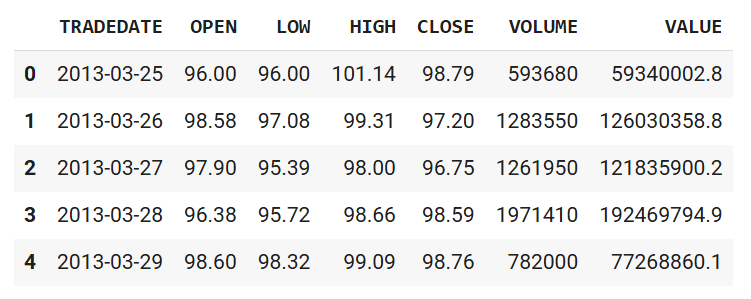
\includegraphics[width=1\linewidth]{cost_example}}
\caption{Пример данных биржи об акции эмитента.}
\label{fig:cost_example}
\end{figure}

Получив данные, необходимо проверить целостность. В данном случае я проверял пропуски в данных, и картина получилась не такой хорошей. Как можно видеть на \textquote{Рисунке \ref{fig:miss_percents}}, большая часть акций имеет небольшой процент пропусков, менее 20\%. В 90 бумагах вообще не было пропусков, или они составляли менее одного процента. В данных подсчётах учитывалось отсутствие данных в колонке \textquote{CLOSE} в любой из дней. Тем не менее процент пропусков более 10 уже будет плохо сказываться на достоверности данных при обучении и валидации, особенно если учитывать бумаги, у которых пропуски под 100\%.
\begin{figure}[H]
\center{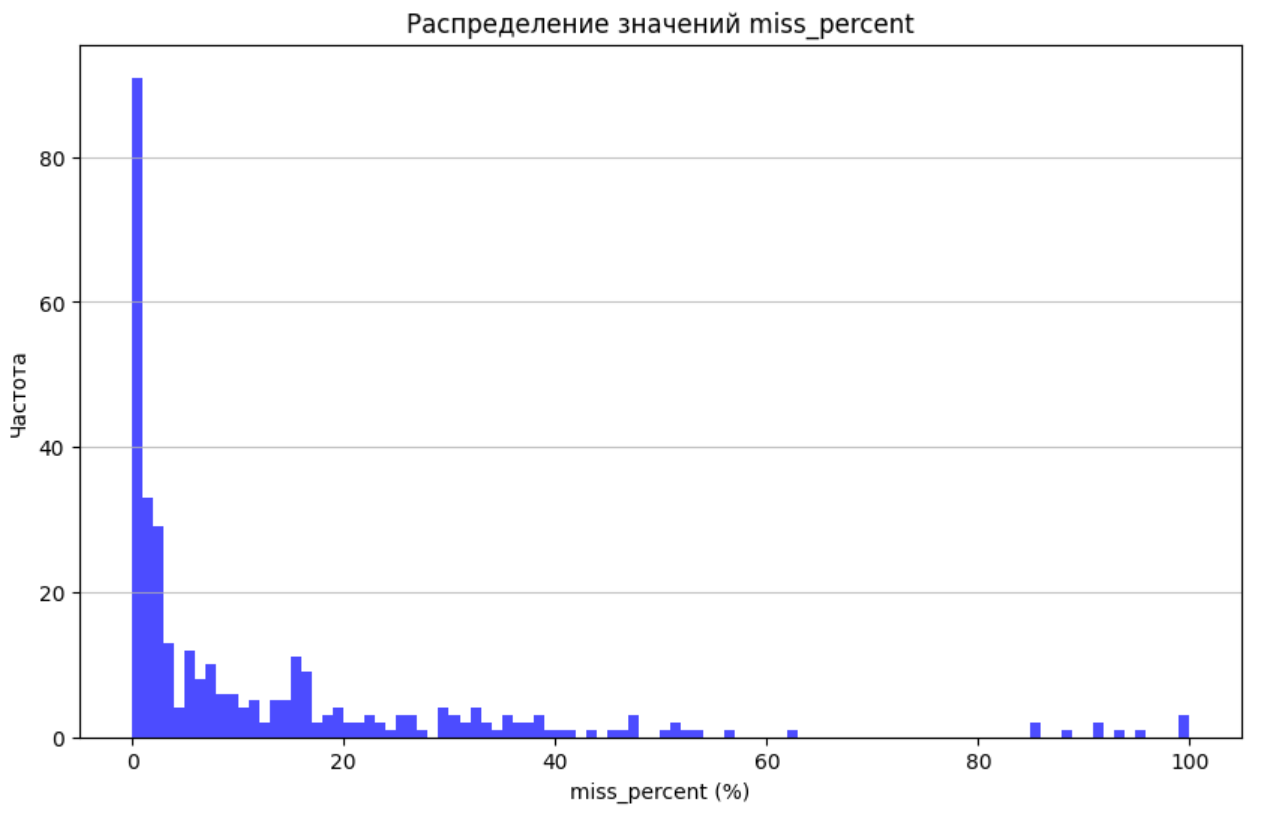
\includegraphics[width=1\linewidth]{miss_percents}}
\caption{Процент пропусков в данных цен акций.}
\label{fig:miss_percents}
\end{figure}

Кроме подсчёта пропусков я получил данные по количеству дней для каждой из бумаг. На \textquote{Рисунке \ref{fig:row_count}} видно, что есть аномальный выброс данных на значении 2624. Это значит, что по какой-то причине у очень большого количества бумаг данные были получены не ранее определённого дня, примерно 10.5 лет назад. Не знаю, почему могло такое произойти, но приходится работать с этим. Предположительно, по многим бумагам данные просто не сохранились на Мосбирже, или же при какой-то активности с ними данные более ранних цен были утеряны.
\begin{figure}[h!]
\center{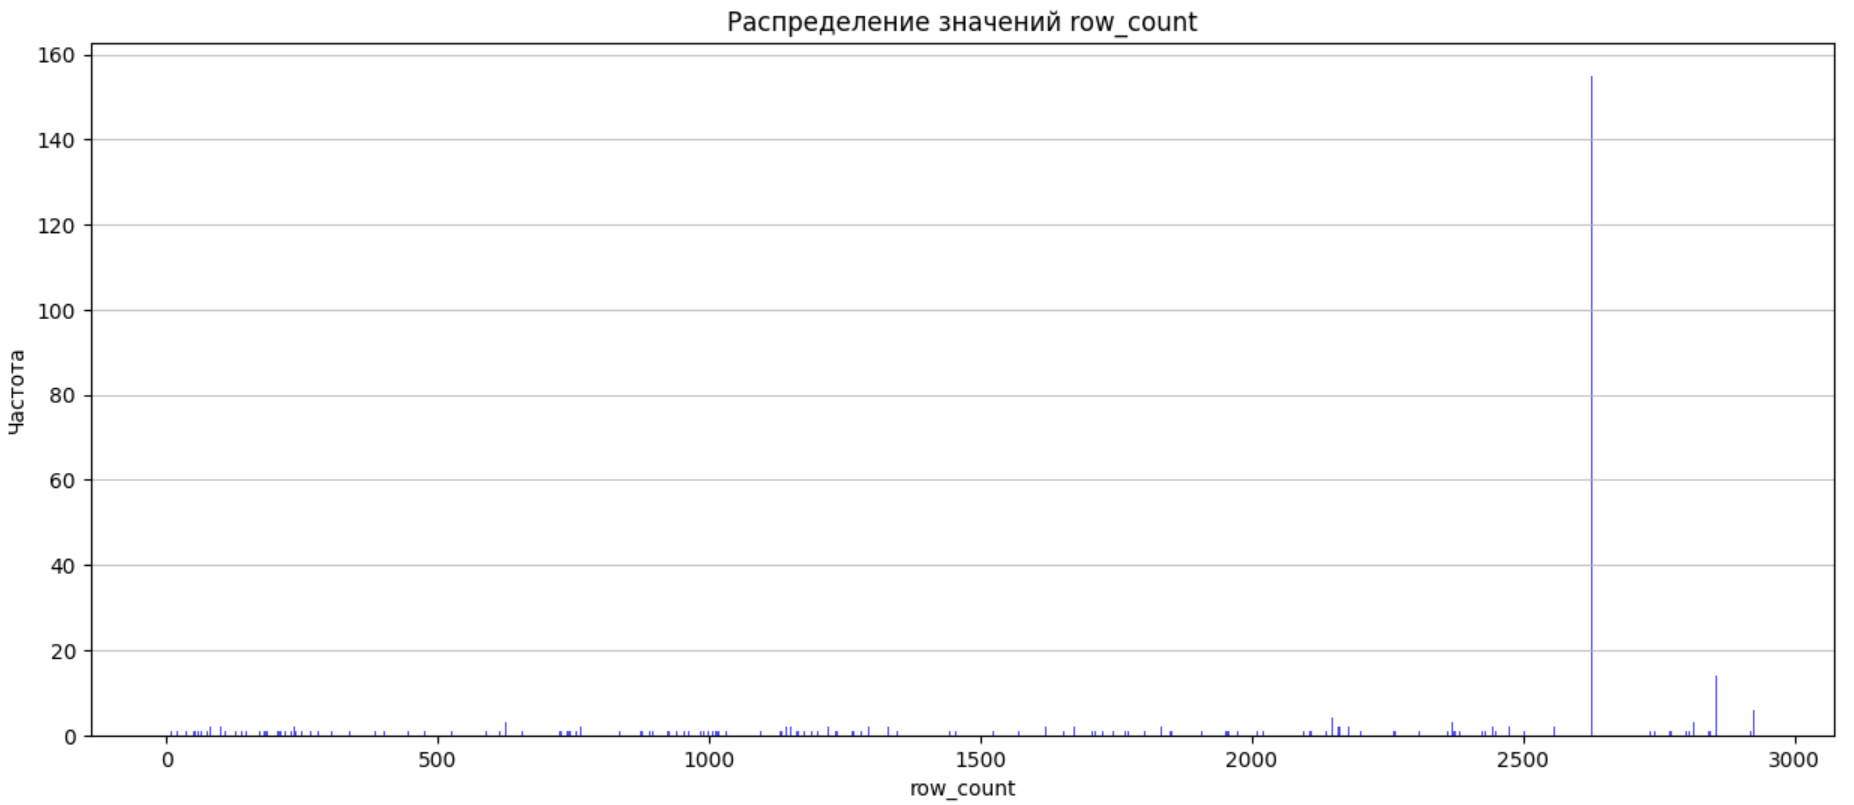
\includegraphics[width=1\linewidth]{row_count}}
\caption{Число дней известных для каждой из бумаг.}
\label{fig:row_count}
\end{figure}

Очевидно, что пропуски в начале данных тяжело заполнить какими-то правдоподобными значениями, это слишком трудно, ведь даже не на что опереться, поэтому я решил избавиться от них. После их устранения средний процент пропусков снизился с 12.87\% до 12.23\%, что не выглядит существенным улучшением. Если смотреть отдельно на бумаги, то минимальным улучшением было 0.01\% или вообще без изменений, потому что не все акции имели пропуски, ну или они были не в начале последовательности. А вот лучший результат получился 84.4\%

Простое удаление начальных пропусков позволило немного уменьшить их процент в акциях, что видно на \textquote{Рисунке \ref{fig:miss_percents_change}} или на \textquote{Рисунке \ref{fig:miss_percent_less_10_change}} с изменениями до 10\%.
\begin{figure}[H]
\center{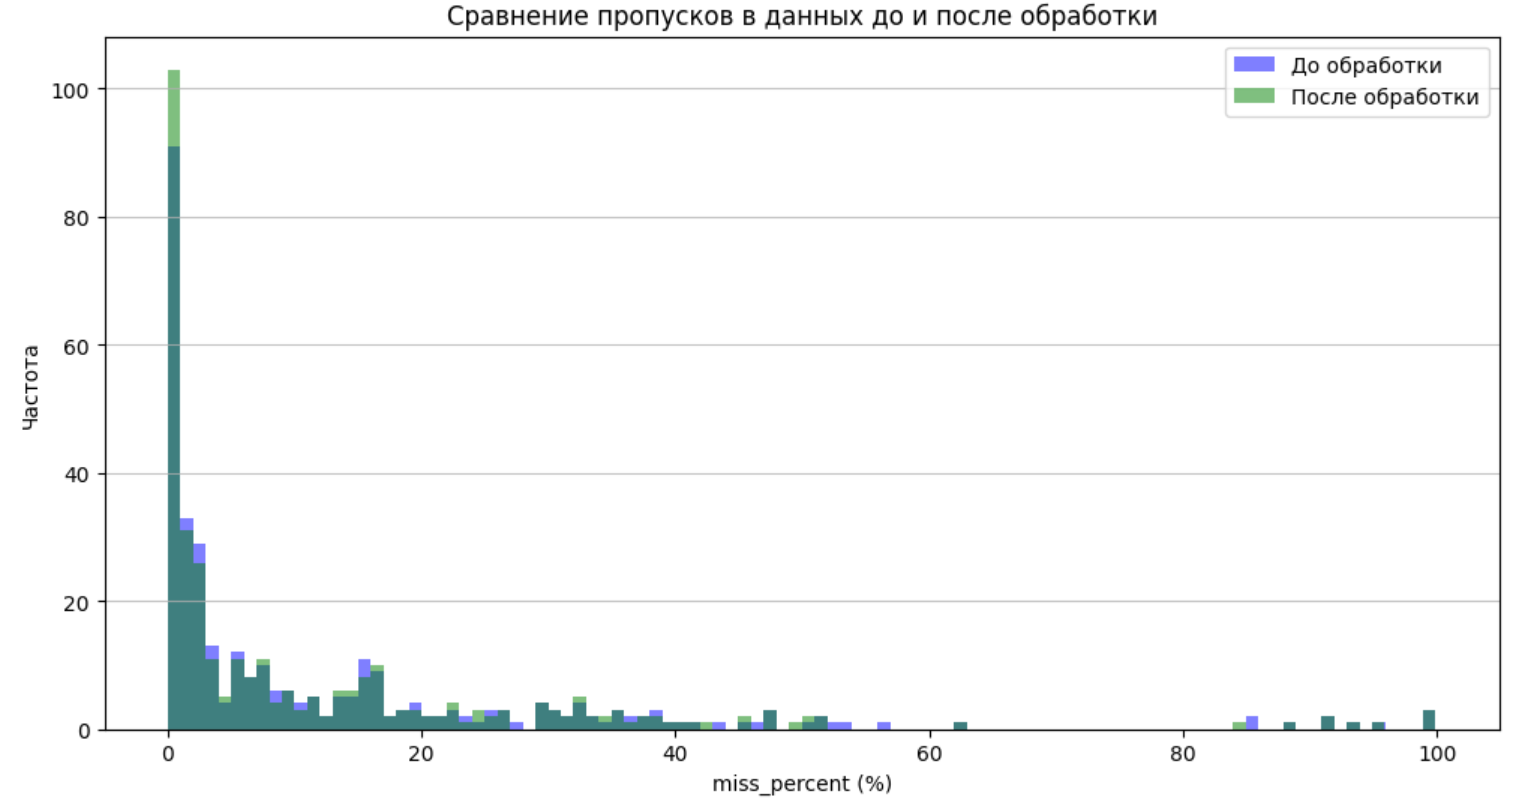
\includegraphics[width=1\linewidth]{miss_percents_change}}
\caption{Изменение процента пропусков в данных цен акций.}
\label{fig:miss_percents_change}
\end{figure}
\begin{figure}[H]
\center{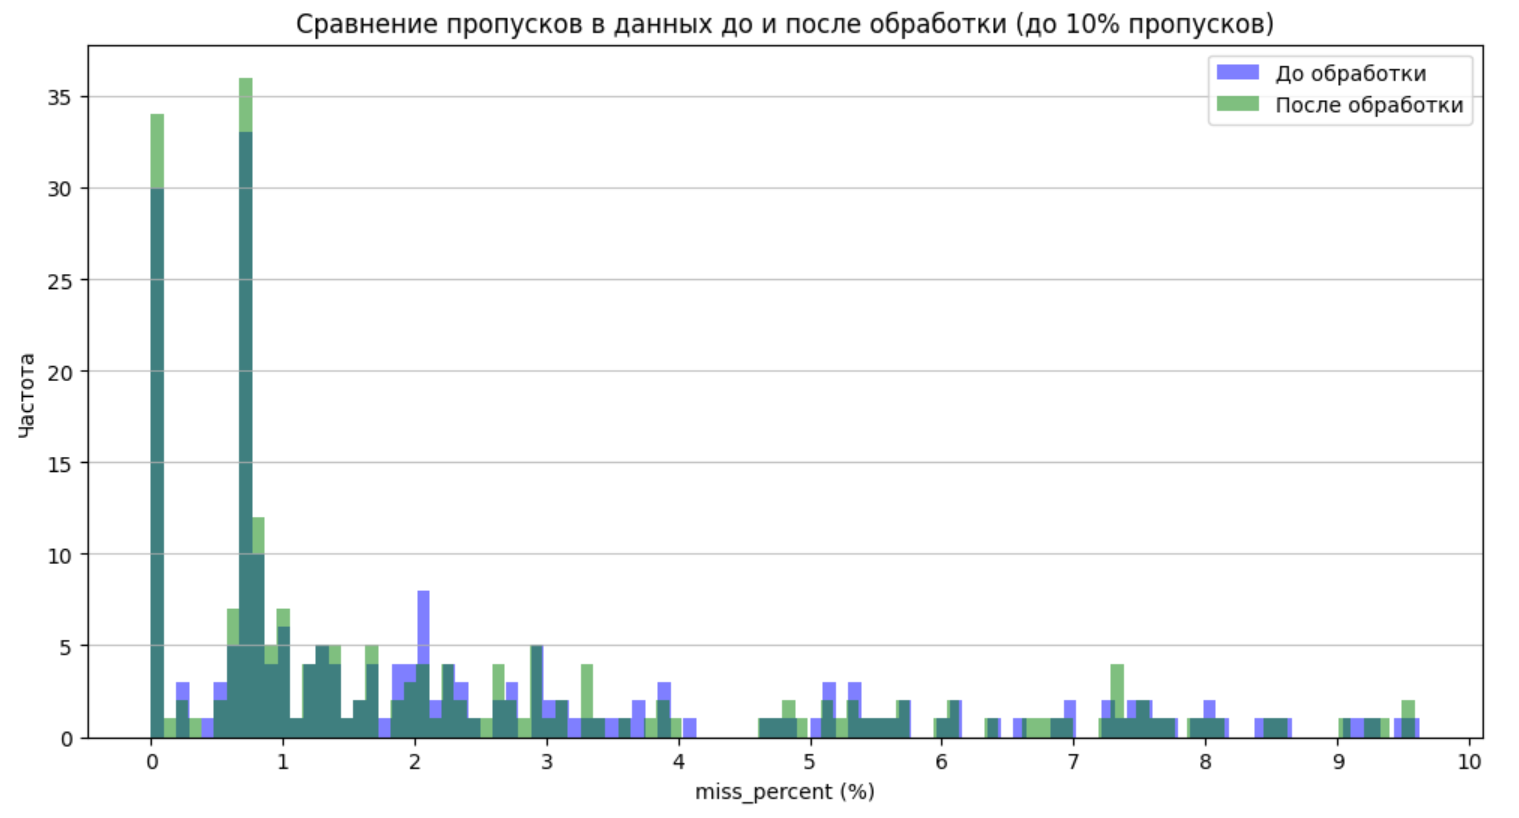
\includegraphics[width=1\linewidth]{miss_percent_less_10_change}}
\caption{Изменение процента пропусков в данных цен акций для акций с пропуском менее 10\%.}
\label{fig:miss_percent_less_10_change}
\end{figure}

Кроме того, изменилось и число данных в акциях, как можно видеть на \textquote{Рисунке \ref{fig:row_count_change}}. Даже в тот аномальный день не все акции имели валидные начальные значения, что делает появление такого выброса ещё более странным.
\begin{figure}[!h]
\center{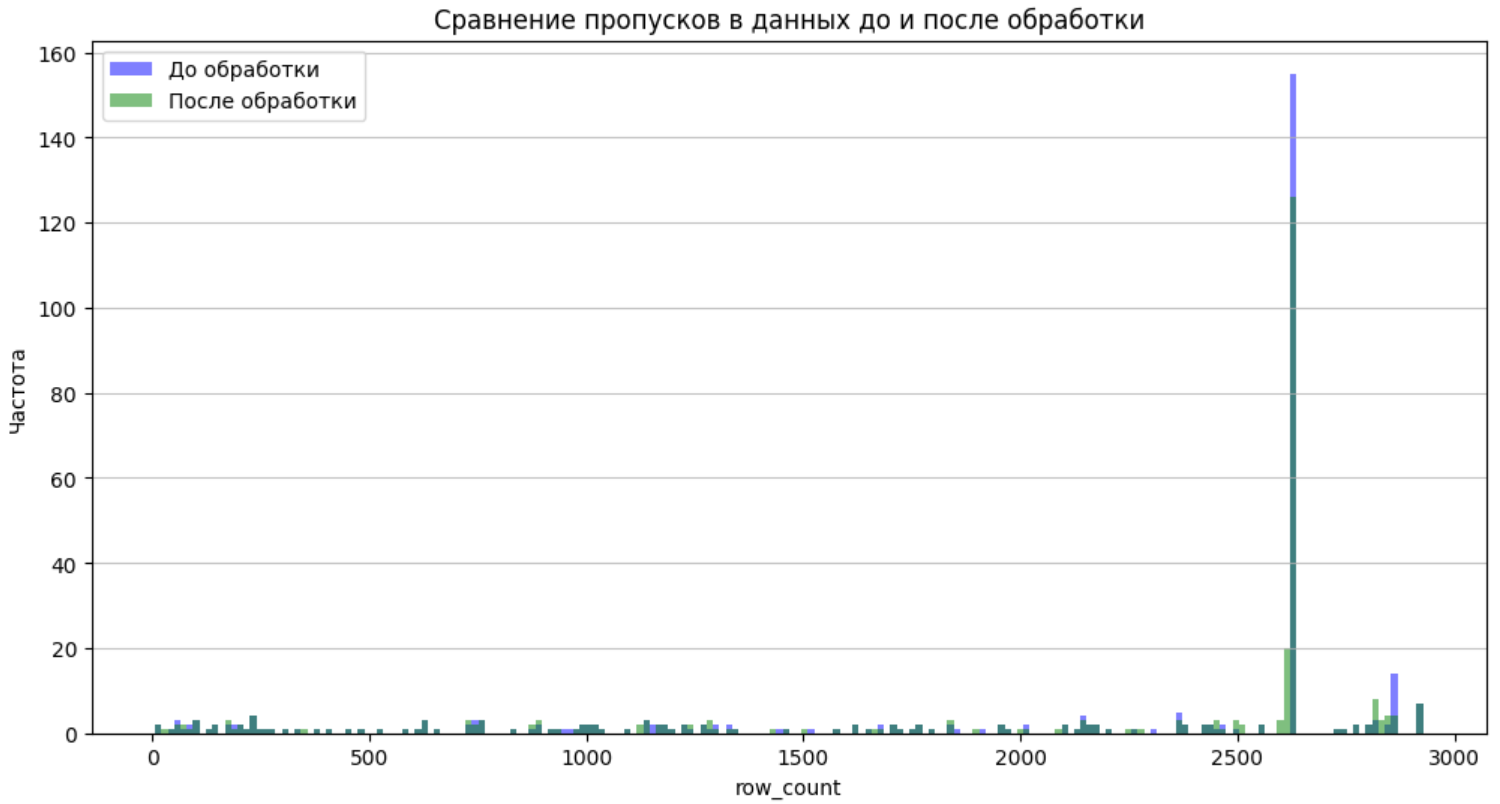
\includegraphics[width=1\linewidth]{row_count_change}}
\caption{Изменение числа дней, известных для каждой из бумаг.}
\label{fig:row_count_change}
\end{figure}

Если говорить об изменении цены акции, то по \textquote{Рисунку \ref{fig:day_cost_change}} можно видеть, что практически вся разница цен получается небольшой, это связано с тем, что сама стоимость бумаг не такая большая, и изменения не так сильны за день. Но некоторые бумаги имеют большую стоимость, поэтому видно, что изменения за день бывают и больше чем 750.
\begin{figure}[H]
\center{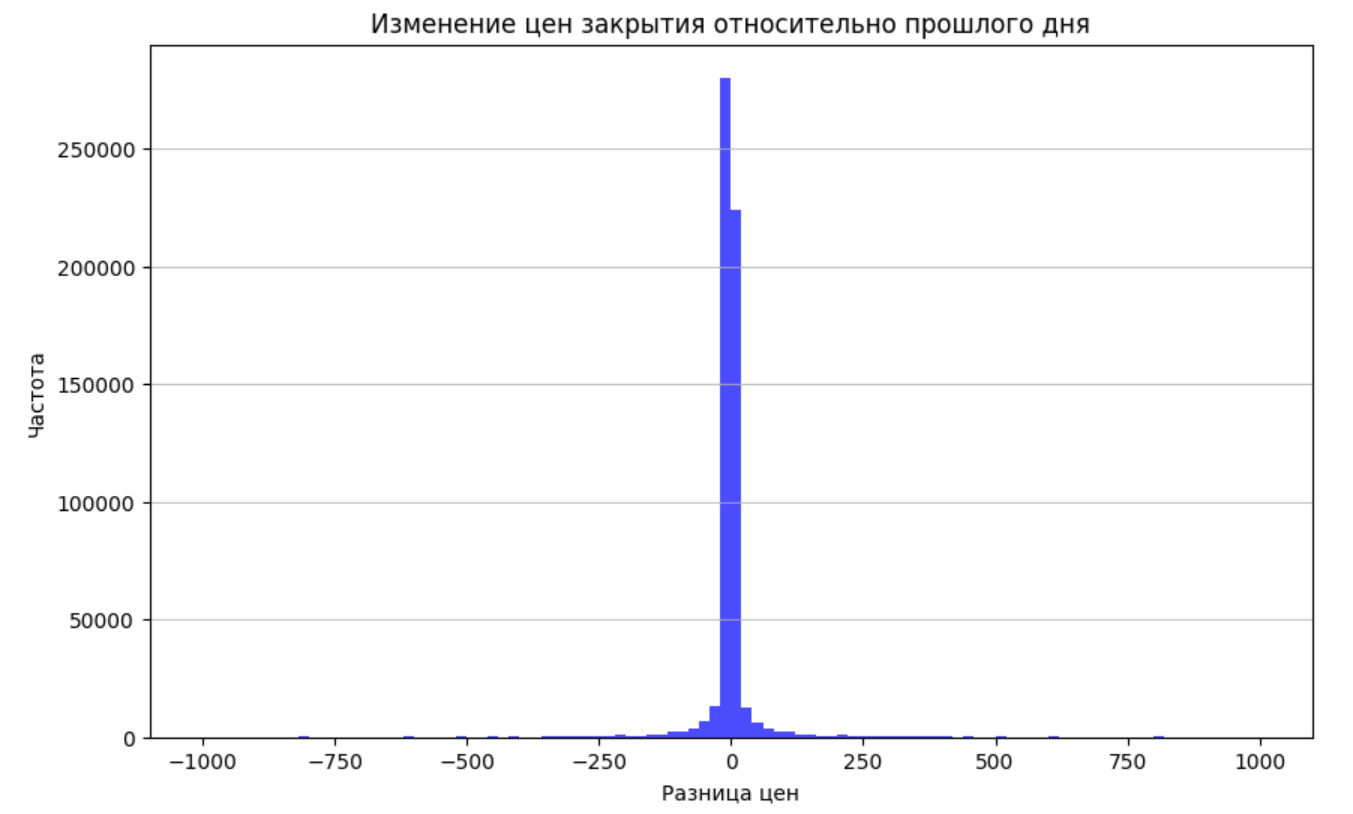
\includegraphics[width=1\linewidth]{day_cost_change}}
\caption{Изменение цен акций за один день.}
\label{fig:day_cost_change}
\end{figure}

Правда, удобнее смотреть изменение цен в процентах, что отображено в \textquote{Рисунке \ref{fig:day_cost_percent_change}}. Видно, что в процентном соотношении цена меняется незначительно, в преобладающем большинстве примерно на половину процента в день. Да, эти графики являются обрезанными по краям, потому что иначе их анализ был бы не таким удобным. Ведь бывают резкие изменения цен акций при новостях, отчётах или тех же дивидендных отсечках.
\begin{figure}[h!]
\center{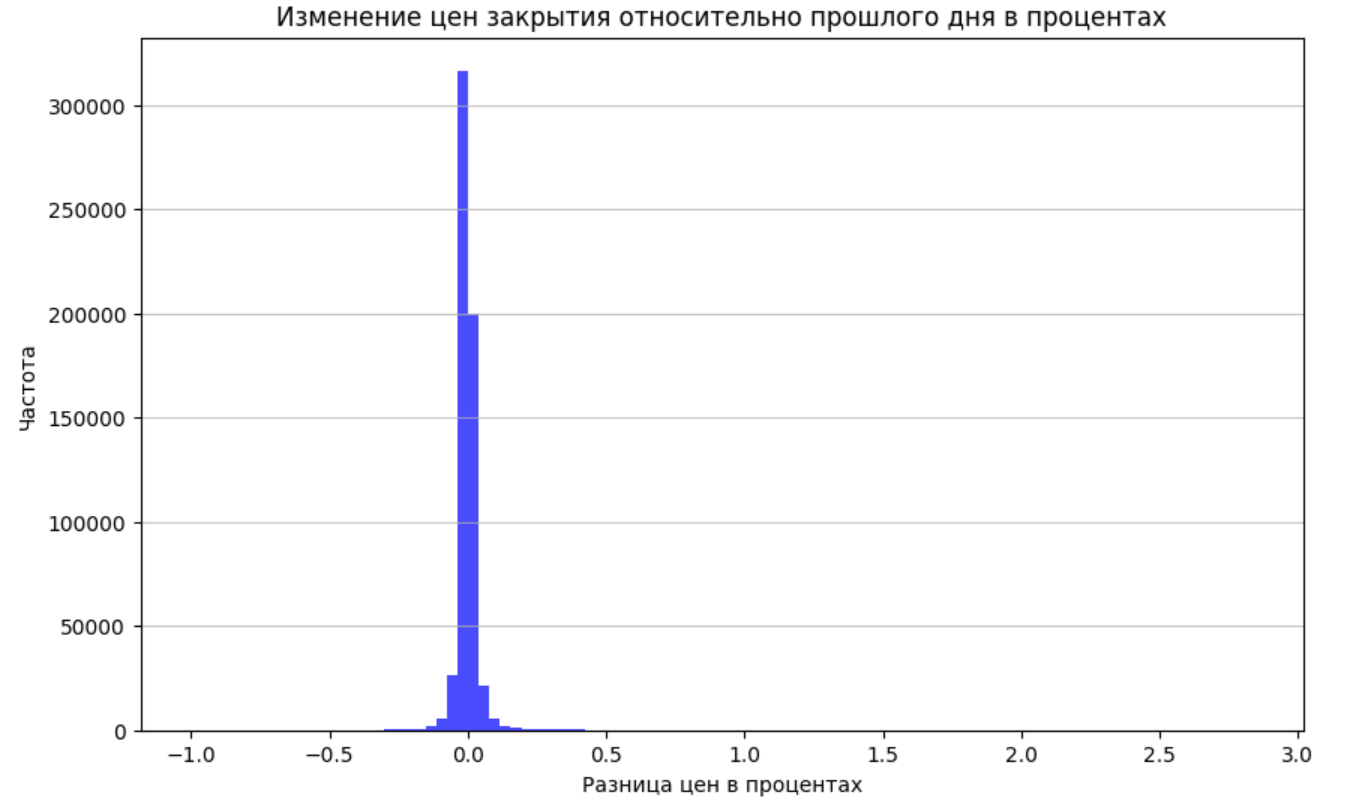
\includegraphics[width=1\linewidth]{day_cost_percent_change}}
\caption{Изменение цен акций за один день в процентах.}
\label{fig:day_cost_percent_change}
\end{figure}

Кроме всего выше написанного, хочу представить графики по числу бумаг в обороте за один день \textquote{Рисунок \ref{fig:volume_count}} и по их стоимости \textquote{Рисунок \ref{fig:value_count}}, из чего следует, что примерный оборот в день составляет около 50 миллиардов.
\begin{figure}[H]
\center{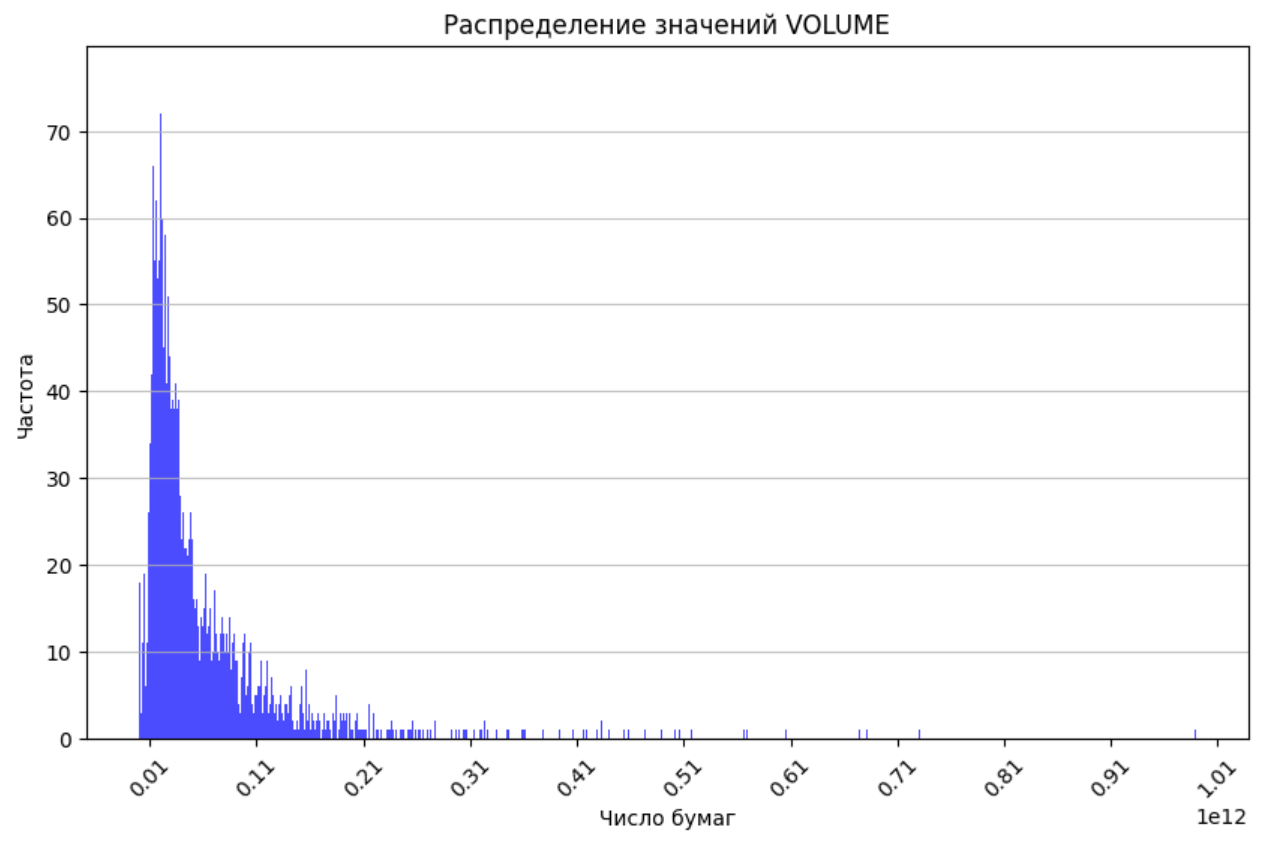
\includegraphics[width=1\linewidth]{volume_count}}
\caption{Оборот торгов за день.}
\label{fig:volume_count}
\end{figure}
\begin{figure}[H]
\center{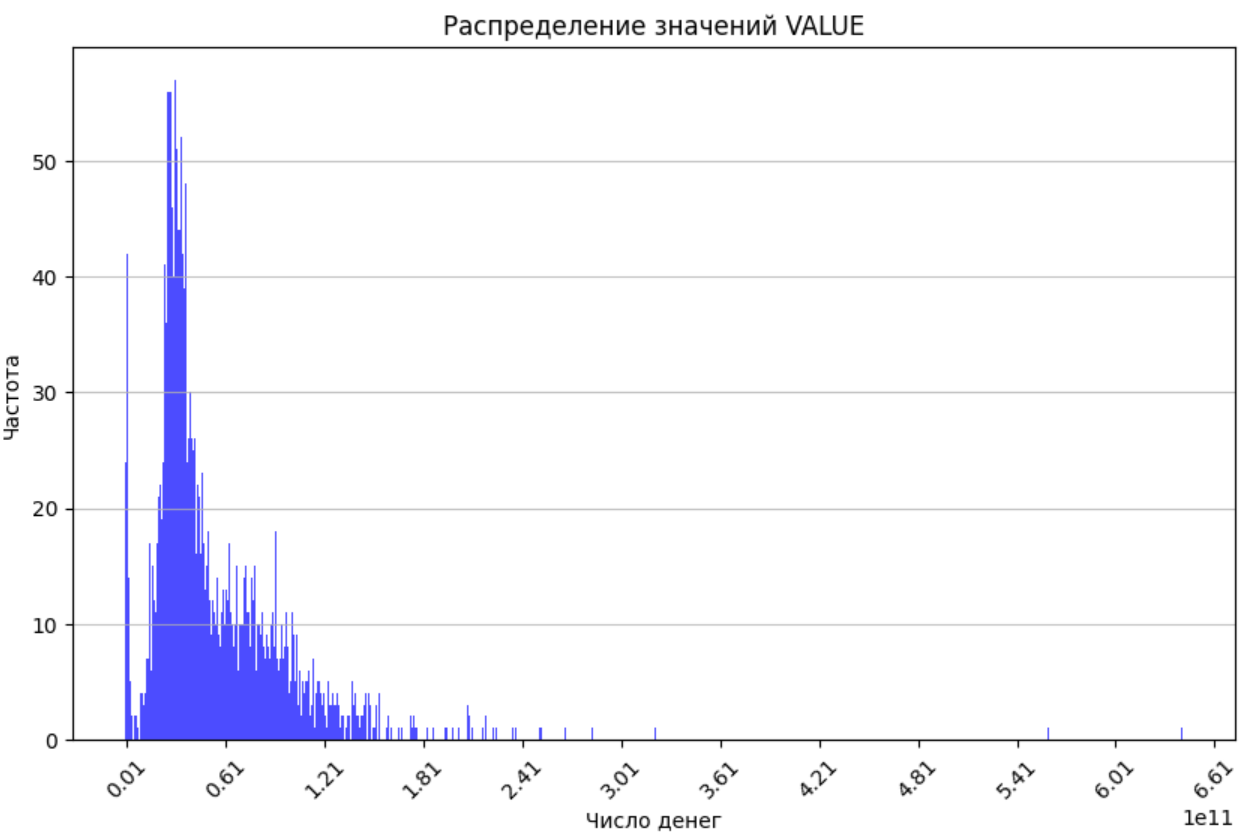
\includegraphics[width=1\linewidth]{value_count}}
\caption{Объём торгов за день.}
\label{fig:value_count}
\end{figure}

Для получения хоть сколько-то реальных предсказаний пришлось отказаться от всех бумаг, пропуски в которых составляли более 10\%. Таким образом, их общее число сократилось до 215 единиц.

После чего оставался последний шаг в предобработке данных - это избавление от пропусков. По различным причинам большинство акций имеют пропуски, хотя хранят день, как будто полноценно торговались, что можно видеть на \textquote{Рисунке \ref{fig:sber_with_misses}}. Скорее всего, в данные дни намеренно приостанавливались торги, что и повлияло на такие разрывы.
\begin{figure}[h!]
\center{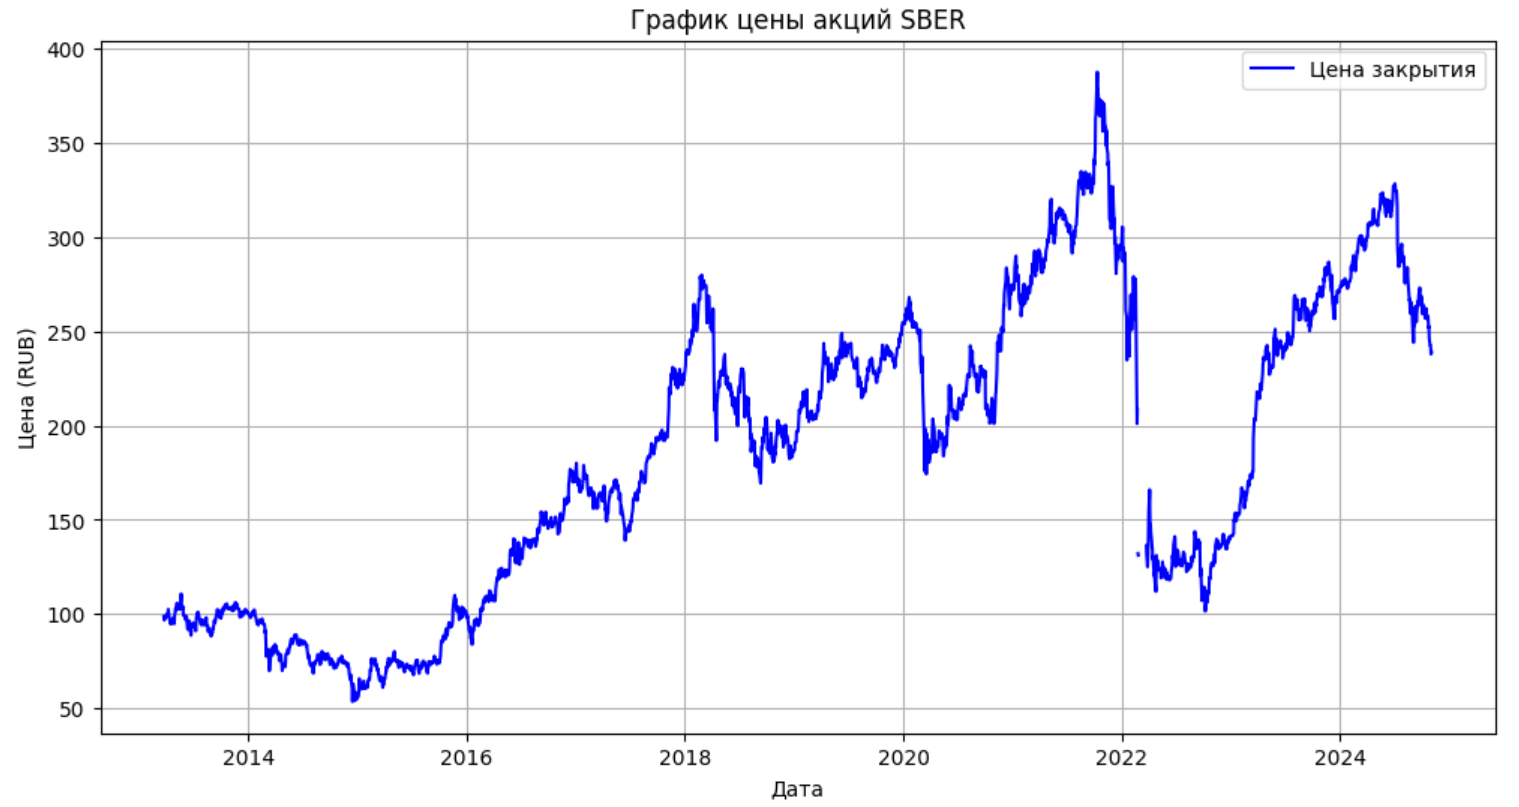
\includegraphics[width=1\linewidth]{sber_with_misses}}
\caption{Цена закрытия акции Сбера.}
\label{fig:sber_with_misses}
\end{figure}

Для избавления от пропусков я для всех бумаг создал скрипт по их заполнению, используя линейную интерполяцию. Так, например, акция с тикером RKKE имела более 8\% пустых значений. Выполнив программу, я получил результат как на \textquote{Рисунке \ref{fig:rkke_interpolate}}, на котором можно видеть прямые участки, которые были добавлены с помощью заполнения. Можно было бы попробовать придумать способ получше для заполнения пропусков, но это сильно усложняет, заставляет рассматривать каждый случай отдельно и сбивает нас с поставленной задачи.
\begin{figure}[!h]
\center{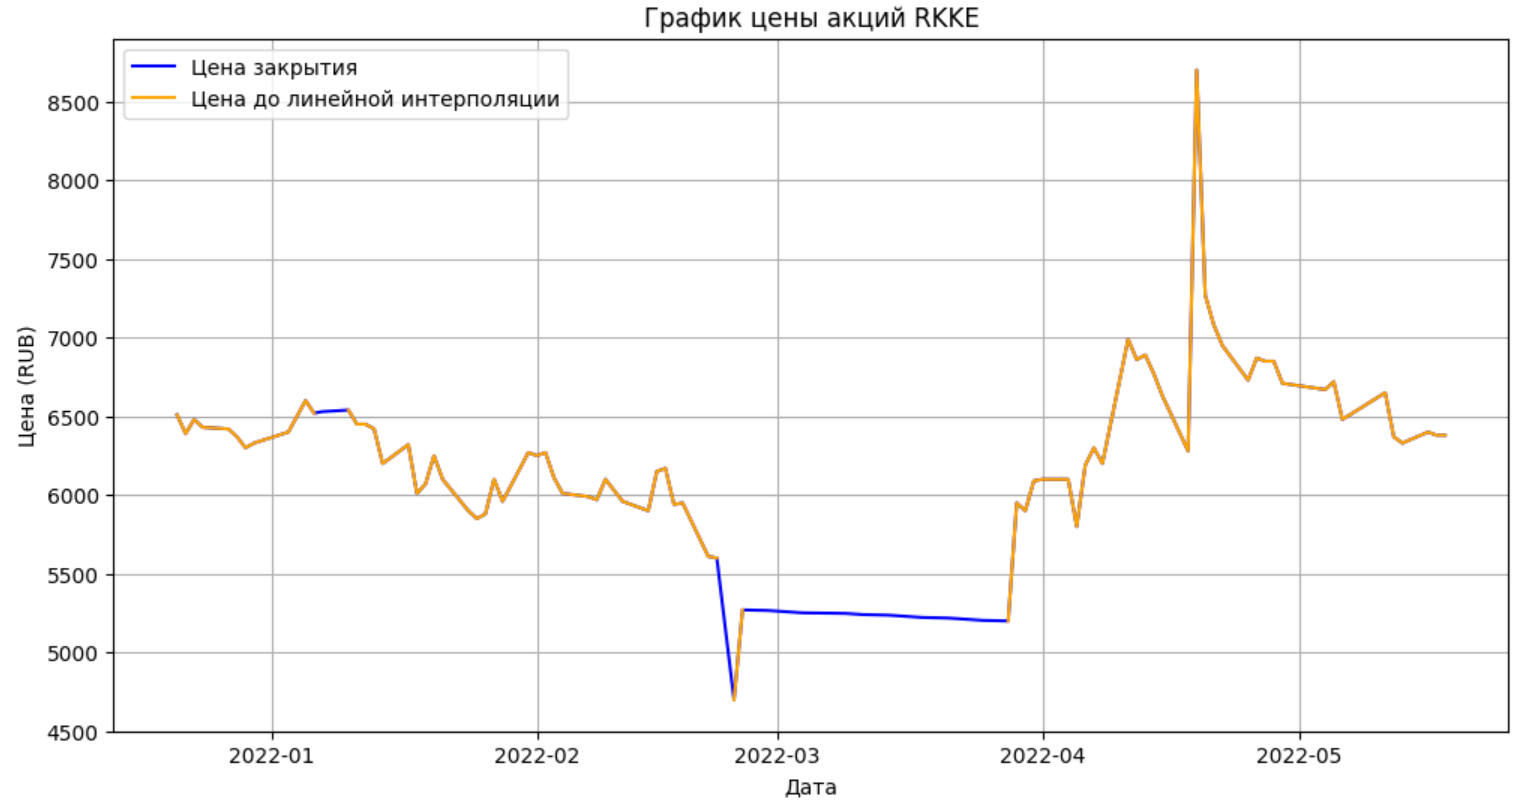
\includegraphics[width=1\linewidth]{rkke_interpolate}}
\caption{Заполнение линейной интерполяцией.}
\label{fig:rkke_interpolate}
\end{figure}

В данной главе я рассказал, как собирал данные по ценам акций, обучение на которых будет позже. Предоставил анализ по распределению, пропускам и выявленной мною информации. И ещё предобработал полученную информацию, подготовив её к следующим действиям.

\subsection{Новости по акциям}

Для получения новостей я начал изучать доступные источники. Посмотрев различные сайты, статьи и массивы данных на Kaggle \cite{kaggle}, я не нашёл того, что меня бы устроило. В основном данные были неактуальны для руссийского информационного поля, их было не так много или они были в малом количестве, поэтому я решил собрать свою базу новостей.

Для выбора источника я рассматривал несколько сайтов. В их число входили РИА \cite{ria}, БКС \cite{bcs}, РБК \cite{rbc}, Smart-lab \cite{smartlab}, MOEX \cite{moex}, Finam \cite{finam} и Investing \cite{investing}. При выборе фаворита я смотрел на удобство получения данных, на полноту, то есть как много и часто появляются новости, и на количество исторических данных.

По итогу я выбрал использование РИА новостей \cite{ria}. Данные там хранятся начиная с 2010 года, каждый день было от 200 до 900 новостей, и способ получения данных был достаточно понятен. Да, на некоторых источниках можно было найти новостные данные конкретно по отдельным эмитентам, что могло бы упростить задачу, но я хотел получать больший набор данных, чтобы можно было выявить влияние информации на различные бумаги.

После того как я определился с выбором, я начал получать данные. Изначально мне было необходимо получить ссылки на сами новости, потому что они выдавались порционно по 20 штук на каждый из дней отдельно, например, как в источнике \cite{rialinks}. К сожалению, не все ссылки были читаемыми, и была трудность с количеством обращений на сайт, но мне удалось получить более двух миллионов ссылок.

Следующим этапом было получение уже самих новостей. Для этого я обращался по каждой из ссылок из предыдущего этапа и считывал содержимое. Я всё так же боролся с 429 ошибкой о превышении числа запросов за единицу времени. При получении страницы с новостью я вычленял из неё всю нужную информацию: заголовок, подзаголовок, аннотацию, цитату, текст. На самом деле видов информации там было больше, но я свёл к этим пяти типам. Кроме того, всё что не являлось заголовком или аннотацией, могло встречаться в новости более чем один раз, такие данные я объединял и все имеющиеся ссылки заменял на текст, чтобы не было какого-то странного значения для LLM.

К сожалению, не все новости были для меня полезны. РИА новости часто запускали опросы на разные темы, как на \textquote{Рисунке \ref{fig:opros}}. Такие статьи не несут полезной информации, поэтому я просто сохранял ссылку и никак не обрабатывал информацию из неё.
\begin{figure}[H]
\center{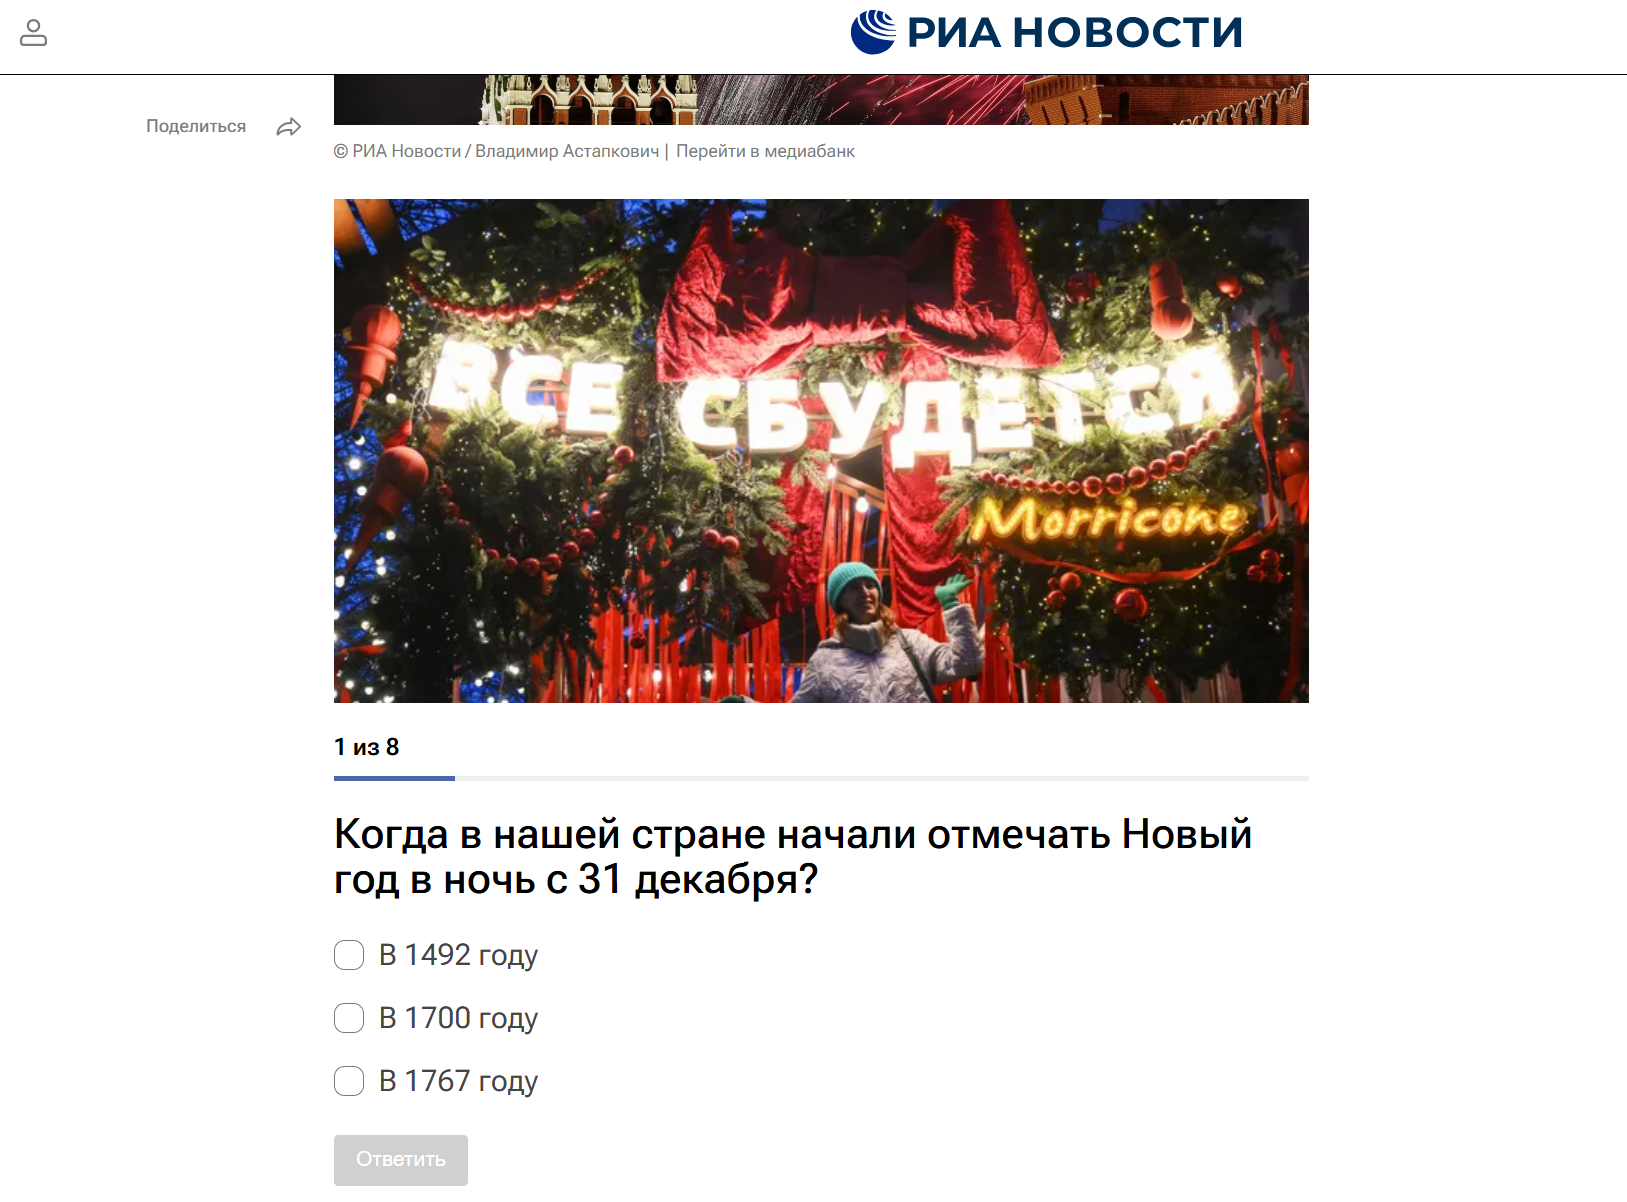
\includegraphics[width=1\linewidth]{opros}}
\caption{Опрос РИА новостей.}
\label{fig:opros}
\end{figure}

Кроме этого, некоторые новости были не такого формата, как преобладающее большинство, например, \textquote{Рисунок \ref{fig:unusial}}. Просмотрев большое количество подобных неподходящих данных, я понял, что они тоже редко обладают какой-то важной информацией. Поэтому я решил не усложнять код и не терять время на этом, такие новости я тоже не использовал в дальнейшем.
\begin{figure}[h!]
\center{
\includegraphics[width=1\linewidth]{unusial}}
\caption{Нестандартный формат РИА новостей.}
\label{fig:unusial}
\end{figure}

Так же встречались новости, которые включали в себя только аннотацию и заголовок. \textquote{Рисунок \ref{fig:annotation}}. Такие новости я на всякий случай записывал как неполные, но их содержание могло быть важным, поэтому, несмотря на такое малое количество информации, я их добавлял в данные для дальнейшей работы.
\begin{figure}[h!]
\center{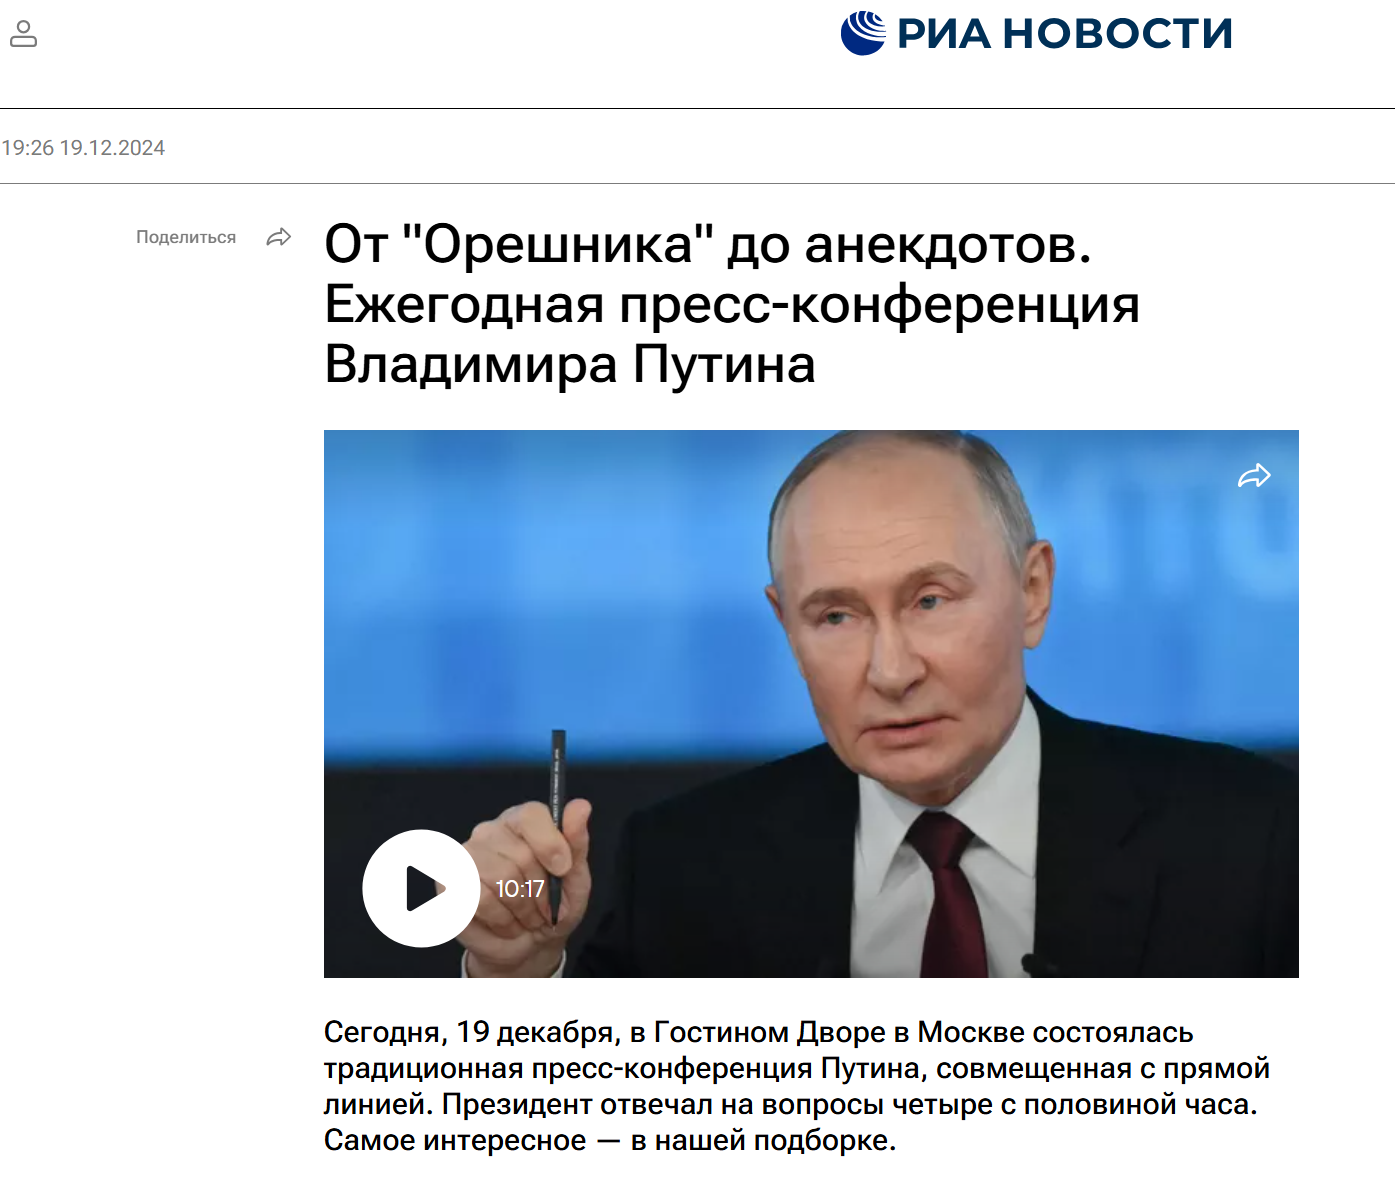
\includegraphics[width=1\linewidth]{annotation}}
\caption{Новость аннотация.}
\label{fig:annotation}
\end{figure}

Все остальные новости были валидными. В общей сложности у меня получилось более 14 лет новостей, из которых чуть меньше 22 тысяч я принимал за неподходящие, что не должно сильно повлиять, ведь это менее одного процента.

Следующим этапом я приступил к оценке новостей. Для этого я начал выбирать модели LLM для использования и источники, где есть к ним бесплатный доступ, потому что у меня было более двух миллионов новостей, и промт запросы включали большое число токенов, обычно из этого и строится цена обращений. В качестве сервиса я нашёл, на то время бесплатный, SambaNova \cite{sambanova}. Доступ был без ограничений, не считая число запросов, с чем я справился. Но что более важно, там не было ограничений из-за моего использования из России.

Для использования их мощностей я получил API ключ и начал тестирование их моделей. Лучшим вариантом для меня стала модель \textquote{Meta-Llama-3.3-70B-Instruct}. На тот момент она была второй по мощности, но обрабатывала в разы больше запросов за единицу времени. Кроме этого, я протестировал её на своих примерах с положительными, отрицательными и нейтральными новостями, и её ответы мне понравились.

Для получения наилучшего результата я создал промт, основными особенностями которого были следующие части:

\begin{enumerate}
  \item Модель является опытным аналитиком с большим стажем на рынке и хорошо разбирается в новостях и их влиянии на российские компании.

  \item Хорошо понимает специфику российской аудитории, реакцию людей на новость и как на какую компанию может это повлиять.

  \item Модель получает все тикеры, которые я собрал ранее, 215 штук, и может предложить свои, в случае дальнейшего обучения.

  \item Обращает внимание на даты новостей и учитывает, есть ли влияние на российский рынок вообще.

  \item Есть описание, как передана новость (заголовок, текст и другое), и предоставлена новость.

  \item Ожидаемый ответ в виде тикера, важности новости для этой компании, сектора компании и причины, почему была выбрана именно такая важность этой новости для данного эмитента.

  \item Важность должна быть от -1 до 1.

  \item Учитывать возможное влияние не только на описанную компанию, но и на конкурентов или союзников из того же сектора или зависимых.
\end{enumerate}

Как я описал ранее, меня устраивали её ответы, то есть и важность, и приведённая причина соответствовали новости. В качестве примера были такие результаты.

Важность 0.542, причина: \textquote{Новость о создании газового хаба в Турции может увеличить поставки газа в Европу, что положительно скажется на компании Газпром}. Как можно видеть, в условиях давления на российский экспорт возможность создания хаба в Турции является большим плюсом для Газпрома, ведь эта страна является членом НАТО и входит в состав Евросоюза, то есть таким способом может помочь России продолжить продавать свой газ под другим флагом, не так сильно снижая его стоимость. 

Важность -0.235, причина: \textquote{Снижение цен на газ в Европе может привести к снижению доходов Газпрома}. Ну а вторая новость очевидно негативная для Газпрома. Поставки в Европу снижаются, продолжаются санкции и попытки отказа от всего российского.

Завершающим этапом было преобразование всех данных под каждый тикер компании, ведь было бы неудобно для использования обращаться к каждому дню и искать среди них нужные значения. Для решения этой задачи я создал скрипт, который выявляет все тикеры и для каждого из них сохраняет минимальную и максимальную важность, выявленную за день, время, в которое эти новости были опубликованы, общее количество новостей за день и их среднюю важность.

В данной главе я описал, как выбирал, получал и обрабатывал новости по желаемым эмитентам. Как их оценивал и предобрабатывал для дальнейшего обучения на них. В результате я получил файлы в облачном хранилище для каждого тикера с необходимой мне информацией на каждый из доступных дней. 

\section{Модели}

\subsection{Метрики}

Для оценки моделей, основываясь на опыте предыдущих работ, мною было выбрано две метрики.

RMSE \textquote{Рисунок \ref{fig:rmse}} является очень полезным и удобным способом отображения ошибки предсказаний от реальных значений в тех же единицах. Её суть в том, что мы складываем все квадраты разностей реального значения и спрогнозированного, после чего делим на количество предсказаний и извлекаем корень для получения ошибки в тех же значениях. В формуле n - число прогнозов, $y_i$ - реальное значение, \^{y} - прогноз модели.
\begin{figure}[!h]
\center{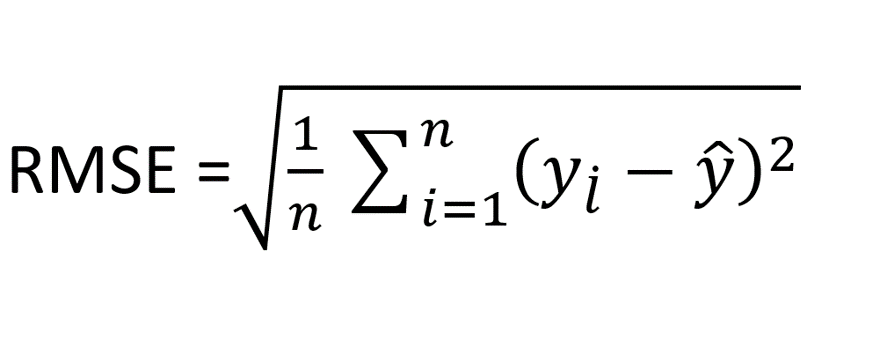
\includegraphics[width=1\linewidth]{rmse}}
\caption{Формула RMSE ошибки.}
\label{fig:rmse}
\end{figure}

MAPE \textquote{Рисунок \ref{fig:mape}} является более наглядным способом для отображения средних ошибок, потому что не привязан к определенным числам, а показывает ошибку в процентах, что может быть полезно, когда для разных акций цена сильно отличается. Её формула немного отличается: считается сумма модулей всех разностей реальных значений и предсказаний, деленных на реальное значение, происходит умножение на 100\% и деление на количество предсказаний. В таком случае мы и получаем процент средней ошибки на всех предсказаниях. В формуле n - число прогнозов, $y_t$ - реальное значение, \^{y} - прогноз модели.
\begin{figure}[!h]
\center{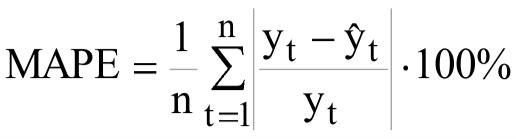
\includegraphics[width=1\linewidth]{mape}}
\caption{Формула MAPE ошибки.}
\label{fig:mape}
\end{figure}

Но, к сожалению, временные ряды, по моему мнению, считать чисто по этим формулам было бы неверно. Ведь очевидно, что любой человек, хоть сколько-то понимающий в фондовом рынке, сделает предсказание на завтра лучше, чем любая самая умная модель, которая попытается предугадать, что будет с бумагой через год. Поэтому в своей работе я считал эти ошибки не на всём промежутке предсказания, а для каждого дня высчитывалась своя ошибка отдельно. Это помогало мне вычислять точность предсказаний на каждый день и смотреть, какая модель лучше показывает результаты на каком промежутке. Если вернуться к моим формулам выше, то для подсчета ошибки просто убирается сумма и деление на число предсказаний, ведь каждый день считается отдельно.

\subsection{По ценам}

Для более точного предсказания я выделил группу бумаг, у которых известны данные о ценах более чем за 5 лет. Это было сделано для получения более точных предсказаний, ведь, как можно было видеть выше на графиках, для некоторых из акций были известны значения цен менее чем за месяц. Я не избавился от них, они тоже были обучены и проанализированы, просто в дальнейшем я буду показывать результаты только по тем 139 компаниям, данные по которым известны более пяти лет.

Биржевой рынок не может обеспечить стабильный поток данных, что сказывается на точности. В нашей стране есть праздники и многое другое, в каких-то неделях может быть 3 рабочих дня, где-то 6, добавляются торги выходного дня и вечерние, чего раньше не было. Такие изменения не позволяют удобно понять цикл, тем более его как-то запрограммировать. Я пробовал использовать более базовые модели, например: ForecastingHorizon, NaiveForecaster, ExponentialSmoothing и AutoETS для прогнозирования именно временных рядов, но из-за описанных проблем приходилось добавлять костыли, и результат мне не нравился.

Тем не менее, для всех моих итоговых моделей, кроме SARIMAX и LSTM, я использовал общий подход. Он заключался в том, что я брал даты и цены закрытия на каждый из дней. Дату я разбивал на год, месяц и день, для цены закрытия я делал лаги. В этом и заключалась основная сложность и непредсказуемость результатов. В году 365 дней, что уже не точно, а рабочих получается около 247. Следуя из этой, примерно верной, информации, я пробовал добавлять лаги, так у меня получилось 1, 2, 3, 4, 5 для первых пяти дней, 10 для лага в две недели, 21 - месяц, 62 - три месяца, 124 - полгода, 247 - год, но цикл может быть и более года, рынок может быть как медвежьим, так и бычьим. Поэтому я добавил ещё лаги на полтора, два и три года. Кроме этого, мне приходилось подчищать данные лагов, чтобы не было такого, что для предсказания на третий день использовалось реальное значение второго дня.

Алгоритм в основном сводился к следующему решению. Я определял параметры для поиска лучшей модели. Проходился по каждому из тикеров. Добавлял лаги, разбивал дату, производил деление на тренировочную и тестовую части. Выполнял нормализацию, используя MinMaxScaler. И начинал GridSearchCV обучение, где таргетом было целевое значение, обучение было направлено на уменьшение RMSE ошибки, а за разбиение отвечал TimeSeriesSplit, который делил на 5 частей. После завершения обучения я итеративно на каждый день делал предсказания и считал ошибки. Для всех, кроме первого дня, я дополнял данные пустых лагов полученными ранее предсказаниями, чтобы третий день считал, что во второй день цена была равной той, что прогнозирует модель. После чего вся необходимая информация сохранялась в облачное хранилище.

\subsection{С использованием новостей}

Для предсказаний с новостями пришлось немного усложнить алгоритм. Во-первых, на каждый из дней добавлялись данные с информацией о новостях (максимальная и минимальная важности, их время, количество новостей и их средняя важность). Если для данной акции не было информации на этот день, то значения важностей устанавливались равными нулю, число новостей - единице, а время - на 14:00, что является примерно серединой торгового дня. После этого время разбивалось на часы и минуты, и добавлялись лаги по той же схеме, что описана в предыдущей главе.

Основным усложнением было то, что новости в будущем также не известны, получается, все добавляемые значения, то есть важности, число, время, должны также прогнозироваться. Таким образом, в предсказании получается уже 9 ожидаемых полей. И во время последнего этапа с оценкой и получением значений на будущие дни от модели лаги по новостям заполняются по тому же принципу, что и лаги по цене.

\subsection{SARIMAX}

SARIMAX (Seasonal Autoregressive Integrated Moving Average with eXogenous regressors) — это мощная модель временных рядов, которая используется для прогнозирования данных, имеющих сезонные компоненты и внешние регрессоры. SARIMAX является расширением модели ARIMA, которая включает в себя сезонные эффекты и возможность добавления внешних переменных.

S (Seasonal): Этот компонент добавляет сезонные эффекты в модель.

AR (Autoregressive): Этот компонент учитывает зависимость текущего значения временного ряда от его предыдущих значений. 

I (Integrated): Этот компонент отвечает за разности временного ряда, чтобы сделать его стационарным. Стационарный ряд — это ряд, у которого статистические свойства, такие как среднее и дисперсия, не зависят от времени.

MA (Moving Average): Этот компонент учитывает зависимость текущего значения от предыдущих ошибок прогноза. Это позволяет модели корректировать свои предсказания на основе прошлых ошибок.

X (eXogenous regressors): Это возможность добавления внешних переменных, которые могут влиять на временной ряд.

Данная модель больше всего отличается от описанного выше шаблона: в ней не используются новости или какие-то ещё поля; необходимы только данные по ценам, но предсказания я так же оценивал ежедневно, чтобы иметь один формат результатов.

В данном случае я не вижу необходимости показывать результаты по отдельным бумагам. Предсказанные ею значения неплохи, но даже на малом промежутке ничего классного нет. Она редко показывают результаты лучше остальных моделей. Хотя у неё есть преимущество в малой требовательности к данным.

Если рассматривать средние результаты по 139 акциям старше пяти лет, то в \textquote{Таблице \ref{tab:sarimax}} видно, что ошибка в первый день в среднем составляет 3\%, а к концу второй недели - уже более 12 с половиной. И дальше результат, очевидно, лучше не будет, что видно на \textquote{Рисунке \ref{fig:sarimax}}, который показывает увеличение ошибки в первый месяц.
\begin{table}[H]
\centering
\caption{Таблица средних ошибок SARIMAX на две недели.}
\begin{tabular}{ |c|c|c| } 
 \hline
 День предсказания & RMSE & MAPE \\ 
 \hline
1 & 82.211 & 3.018 \\ 
 \hline
2 & 154.788 & 5.100 \\ 
 \hline
3 & 254.078 & 6.384 \\ 
 \hline
4 & 314.963 & 6.573 \\ 
 \hline
5 & 268.571 & 6.475 \\ 
 \hline
6 & 374.613 & 8.622 \\ 
 \hline
7 & 486.077 & 11.278 \\ 
 \hline
8 & 641.263 & 12.515 \\ 
 \hline
9 & 692.472 & 12.436 \\ 
 \hline
10 & 612.356 & 12.491 \\ 
 \hline
\end{tabular}
\label{tab:sarimax}
\end{table}
\begin{figure}[!h]
\center{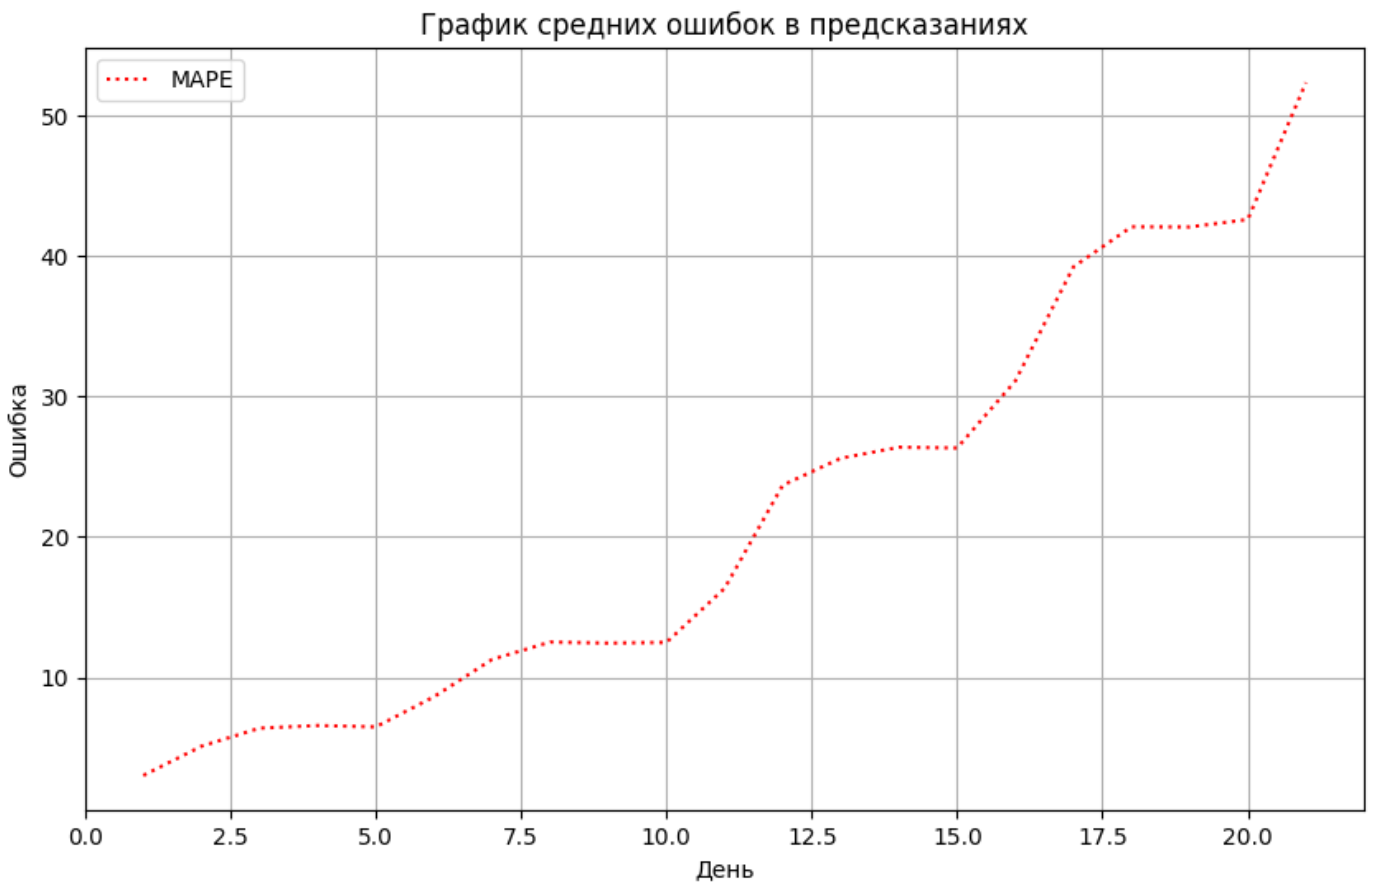
\includegraphics[width=1\linewidth]{sarimax}}
\caption{MAPE ошибка SARIMAX на первый месяц.}
\label{fig:sarimax}
\end{figure}

\subsection{Ridge Regression}

Ridge - это техника, которая применяется в контексте линейной регрессии для борьбы с проблемой мультиколлинеарности и переобучения. Основная идея заключается в добавлении L2-регуляризации к функции потерь, что позволяет контролировать величину коэффициентов регрессии.

Обучение этой модели проходило, как было описано в начале этой большой главы, как без использования новостей, так и с ними. В отличие от SARIMAX количество используемых данных было увеличено, особенно с новостями, и это принесло свои плоды: точность предсказаний у данной модели в среднем лучше, и она чаще дает более точные предсказания. В некоторых случаях она лучше даже на горизонте в полгода и год. Для обучения параметр alpha подбирался в диапазоне от 0.0001 до 10000, а fit\_intercept - либо True, либо False.

Правда, если сравнивать данную модель без использования новостей и с ними, то средние значения получались неожиданными. По \textquote{Таблице \ref{tab:ridge}} видно, что почти во всех случаях точность предсказания лучше у модели без новостей. На самом деле, такое получается во многих моделях, что я объясню в завершение главы.
\begin{table}[H]
\centering
\caption{Таблица средних ошибок Ridge на две недели.}
\begin{tabular}{ |c|c|c|c|c| } 
 \hline
 День предсказания & Ridge RMSE & Ridge + news RMSE & Ridge MAPE & Ridge + news MAPE \\ 
 \hline
1 & \textbf{20.785} & 43.508 & \textbf{1.476} & 1.715 \\ 
 \hline
2 & \textbf{25.420} & 52.559 & \textbf{2.287} & 2.917 \\ 
 \hline
3 & 53.785 & \textbf{43.131} & \textbf{2.959} & 3.619 \\ 
 \hline
4 & \textbf{71.724} & 94.299 & \textbf{3.233} & 3.670 \\ 
 \hline
5 & \textbf{61.794} & 137.609 &\textbf{ 3.672} & 4.413 \\ 
 \hline
6 & \textbf{68.694} & 136.872 & \textbf{4.113} & 5.458 \\ 
 \hline
7 & \textbf{81.128} & 141.974 & \textbf{4.353} & 5.631 \\ 
 \hline
8 & \textbf{99.891} & 164.282 & \textbf{4.766} & 5.861 \\ 
 \hline
9 & \textbf{102.058} & 198.797 & \textbf{4.984} & 6.296 \\ 
 \hline
10 & \textbf{94.851} & 198.242 & \textbf{5.158} & 6.225 \\ 
 \hline
\end{tabular}
\label{tab:ridge}
\end{table}

Также можно посмотреть средние MAPE ошибки на ближайший месяц для обученной модели на \textquote{Рисунке \ref{fig:ridge}} и для обученной с новостями модели на \textquote{Рисунке \ref{fig:ridge_with_news}}.
\begin{figure}[!h]
\center{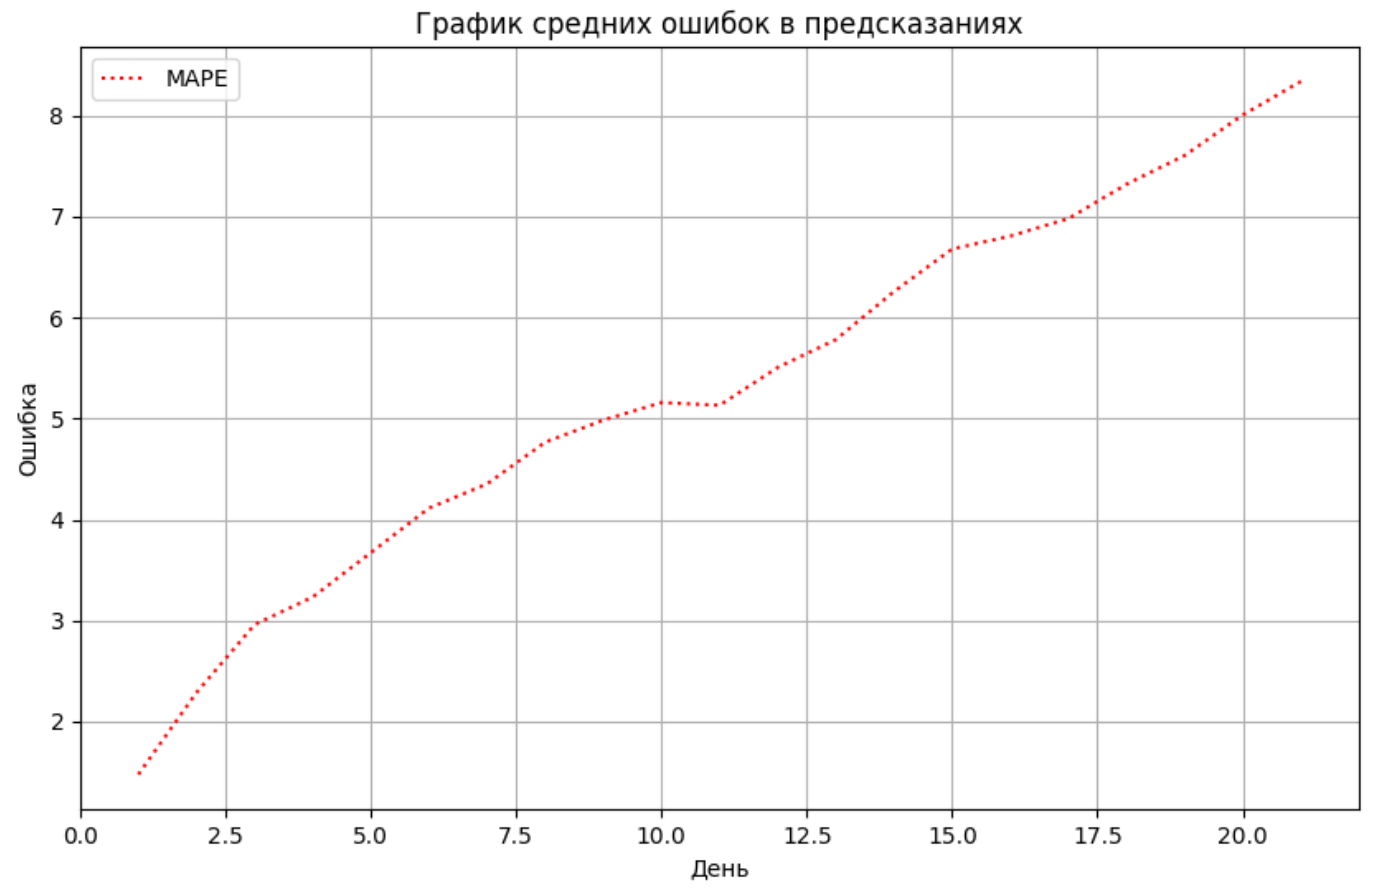
\includegraphics[width=1\linewidth]{ridge}}
\caption{Средняя MAPE ошибка Ridge на первый месяц.}
\label{fig:ridge}
\end{figure}
\begin{figure}[!h]
\center{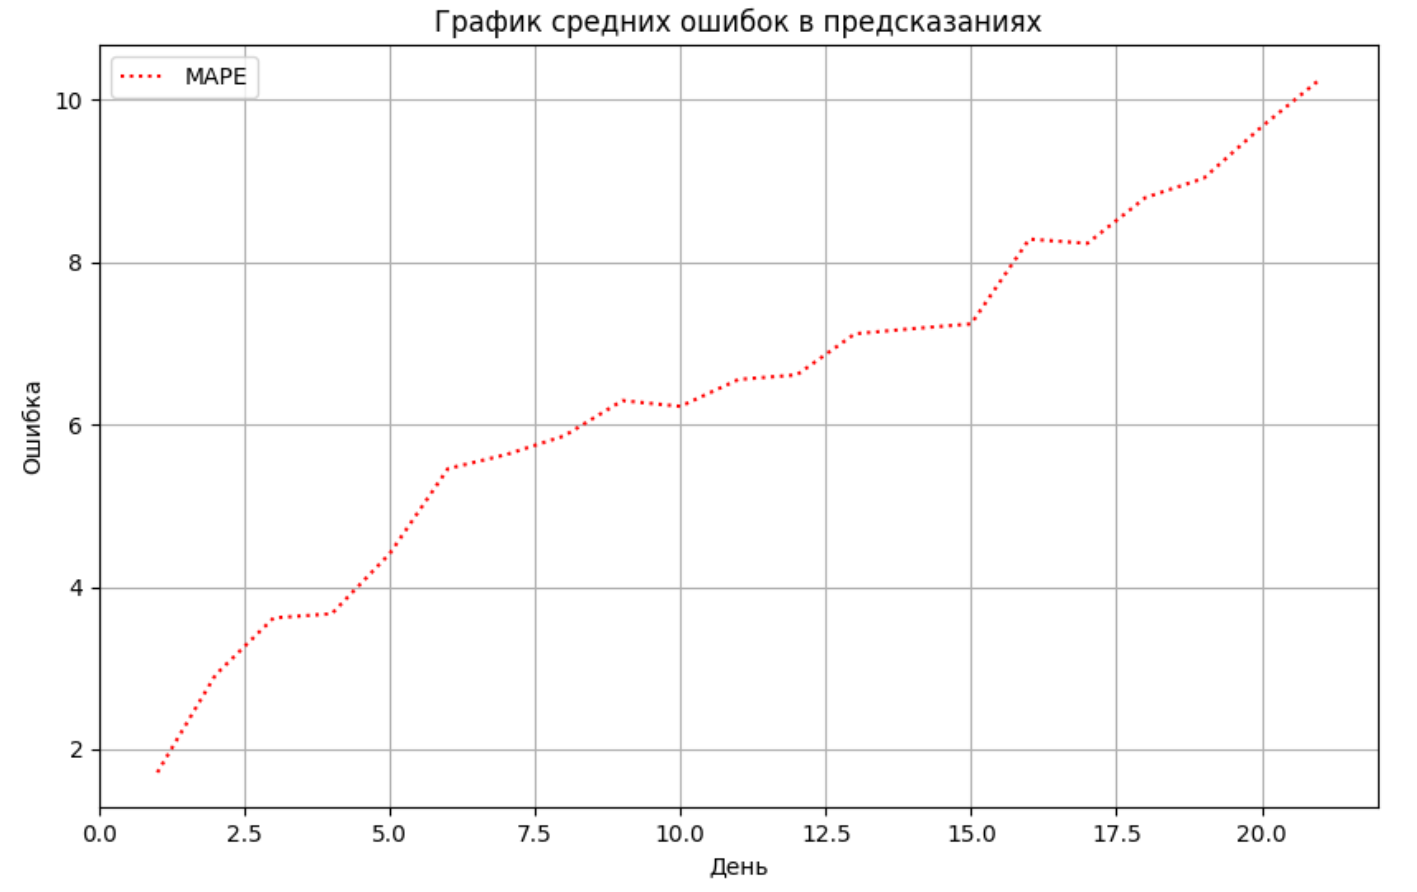
\includegraphics[width=1\linewidth]{ridge_with_news}}
\caption{Средняя MAPE ошибка Ridge с новостями на первый месяц.}
\label{fig:ridge_with_news}
\end{figure}

Более интересно то, что в процентах разница получается от половины до одного процента, но в некоторых случаях RMSE ошибка с новостями в два раза хуже. Предполагаю, что причина в том, что новостная модель чуть хуже прогнозирует значения для акций с большей стоимостью, поэтому проценты почти не отличаются, а абсолютные значения различны в большей степени.

Хотел бы все же повторить, что это среднее значение, то есть для некоторых бумаг новостная модель показывает результаты лучше.

\subsection{Random Forest Regression}

Random Forest - представляет собой ансамблевый метод, который использует множество деревьев решений для принятия более точных решений. Основная идея заключается в том, что несколько деревьев, обученных на различных подмножествах данных, могут давать более надежные прогнозы, чем одно дерево.

Обучение происходило так же, как и для модели Ridge, за тем исключением, что параметрами для выбора были: n\_estimators - [50, 100, 200, 300, 400, 500], max\_features - [log2, sqrt], max\_depth - [None, 10, 20, 30], min\_samples\_split - [2, 5, 10], min\_samples\_leaf - [1, 2, 4], bootstrap - [True, False]

Результаты средних ошибок на превые две недели представлены в \textquote{Таблице \ref{tab:random_forest}}. По ней видно, что в первые дни случайный лес показывает результаты немного хуже, чем у модели Ridge, но после второго дня его средняя ошибка меньше, что ещё лучше заметно на \textquote{Рисунке \ref{fig:random_forest}}. К сожалению, случайный лес с новостями показал не столь хороший результат \textquote{Рисунок \ref{fig:random_forest_with_news}}, думаю, это связано с тем, что получается слишком много признаков относительно данных, что усложняет нахождение зависимостей.
\begin{table}[H]
\centering
\caption{Таблица средних ошибок Random Forest на две недели.}
\begin{tabular}{ |c|c|c|c|c| } 
 \hline
 День предсказания & Forest RMSE & Forest + news RMSE & Forest MAPE & Forest + news MAPE \\ 
 \hline
1 & \textbf{16.721} & 81.013 & \textbf{1.712} & 4.006 \\ 
 \hline
2 & \textbf{18.858} & 83.729 & \textbf{2.443} & 4.654 \\ 
 \hline
3 & \textbf{40.009} & 92.666 & \textbf{2.950} & 5.300 \\ 
 \hline
4 & \textbf{51.671} & 85.500 & \textbf{3.047} & 5.339 \\ 
 \hline
5 & \textbf{46.386} & 95.172 & \textbf{3.340} & 5.794 \\ 
 \hline
6 & \textbf{47.510} & 109.671 & \textbf{3.765} & 6.312 \\ 
 \hline
7 & \textbf{59.279} & 107.751 & \textbf{3.947} & 6.543 \\ 
 \hline
8 & \textbf{71.268} & 89.686 & \textbf{4.334} & 6.820 \\ 
 \hline
9 & \textbf{70.553} & 100.799 & \textbf{4.390} & 7.241 \\ 
 \hline
10 & \textbf{62.685} & 120.310 & \textbf{4.625} & 7.295 \\ 
 \hline
\end{tabular}
\label{tab:random_forest}
\end{table}
\begin{figure}[h!]
\center{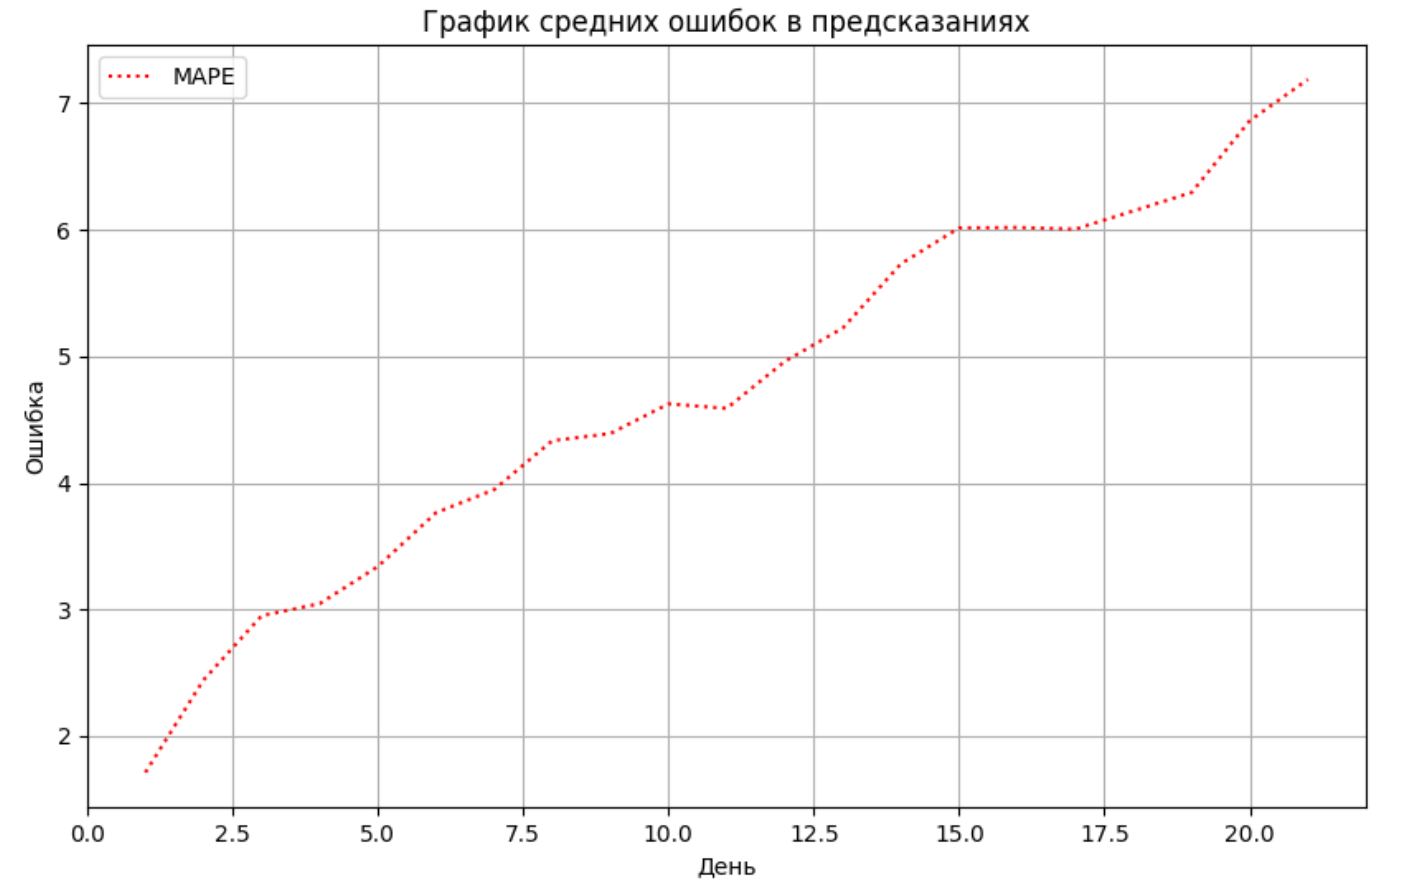
\includegraphics[width=1\linewidth]{random_forest}}
\caption{Средняя MAPE ошибка Random Forest на первый месяц.}
\label{fig:random_forest}
\end{figure}
\begin{figure}[!h]
\center{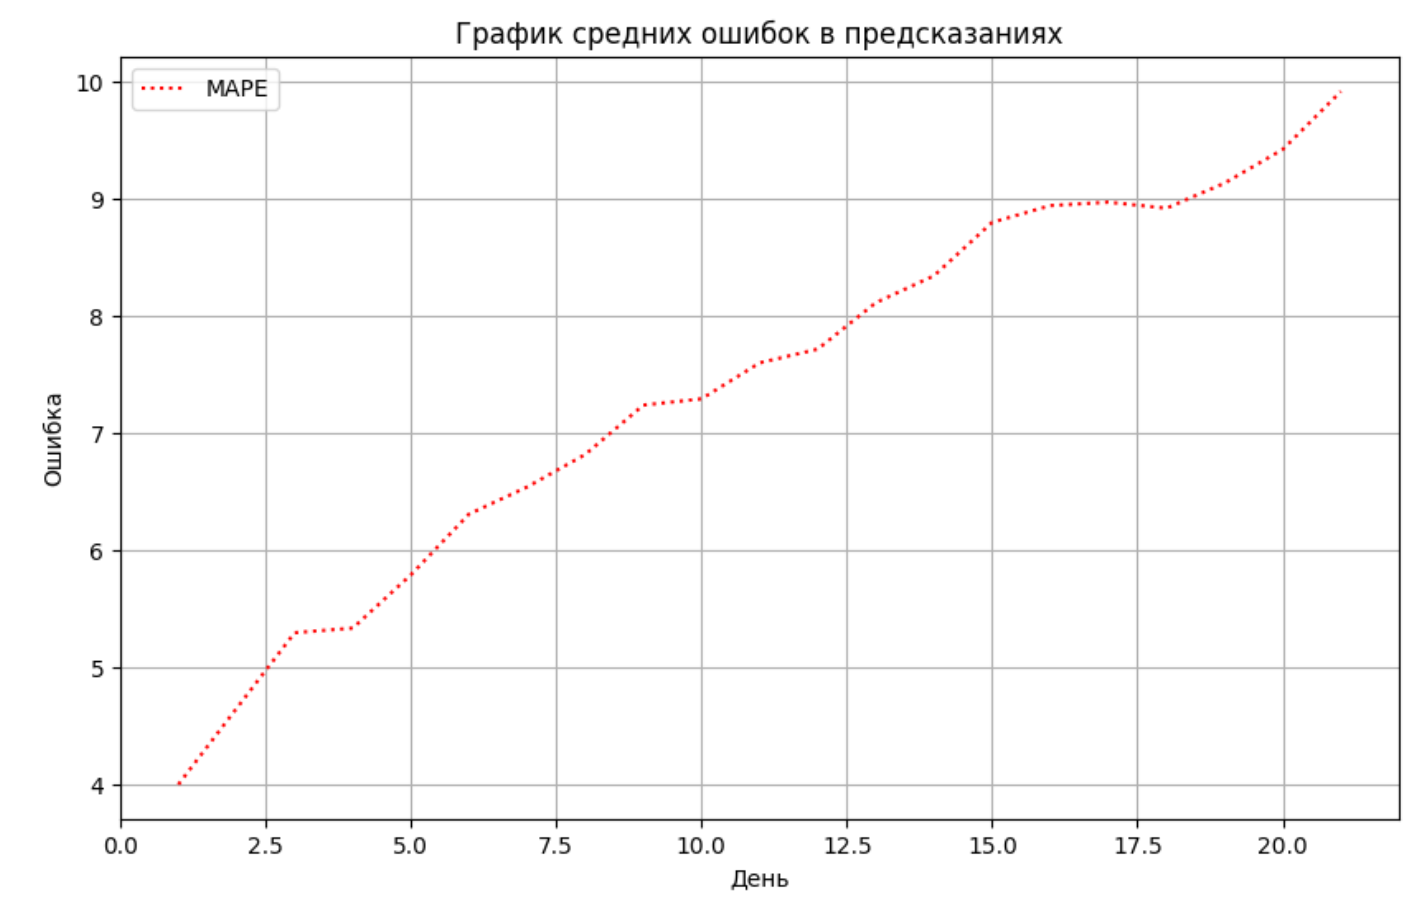
\includegraphics[width=1\linewidth]{random_forest_with_news}}
\caption{Средняя MAPE ошибка Random Forest с новостями на первый месяц.}
\label{fig:random_forest_with_news}
\end{figure}

Случайный лес показывает себя более стабильным в прогнозах на длинный горизонт, даже модель с новостями, имеющая плохие начальные прогнозы, через месяц имеет меньшую ошибку по сравнению с Ridge с новостями.

\subsection{XGBRegressor}

XGBRegressor (Extreme Gradient Boosting Regressor) является частью библиотеки\\XGBoost, предназначеной для реализации алгоритмов градиентного бустинга. Этот метод позволяет создавать предсказательные модели, способные обрабатывать как линейные, так и нелинейные зависимости в данных.

XGBRegressor использует метод градиентного бустинга, который строит модели последовательно, каждая из которых исправляет ошибки предыдущей, что позволяет значительно улучшить точность предсказаний. В отличие от многих других алгоритмов, XGBRegressor включает механизмы регуляризации (L1 и L2), что помогает избежать переобучения модели.

Данная модель обучалась по тому же шаблону, что и две предыдущие, описанному в начале главы. Параметры подбора были следующими: n\_estimators - [100, 200, 300], learning\_rate - [0.01, 0.1, 0.2], max\_depth - [3, 5, 7], min\_child\_weight - [1, 3, 5], subsample - [0.5, 0.7, 1.0], colsample\_bytree - [0.5, 0.7, 1.0], gamma - [0, 1, 5].

Данная модель показала себя не хуже, чем случайный лес. Модель обученная с новостями, хоть и была менее точна в среднем, но оказалась примерно на процент точнее по MAPE, что можно увидеть в \textquote{Таблице \ref{tab:xgboost}}.
\begin{table}[H]
\centering
\caption{Таблица средних ошибок XGBRegressor на две недели.}
\begin{tabular}{ |c|c|c|c|c| } 
 \hline
 День предсказания & XGB RMSE & XGB + news RMSE & XGB MAPE & XGB + news MAPE \\ 
 \hline
1 & 34.296 & \textbf{26.212} & \textbf{1.727} & 2.819 \\ 
 \hline
2 & 48.190 & \textbf{23.163} & \textbf{2.471} & 3.780 \\ 
 \hline
3 & 78.342 & \textbf{30.181} & \textbf{3.002} & 4.229 \\ 
 \hline
4 & 97.238 & \textbf{47.323} & \textbf{3.146} & 4.325 \\ 
 \hline
5 & 91.990 & \textbf{59.053} & \textbf{3.552} & 4.743 \\ 
 \hline
6 & 92.665 & \textbf{45.018} & \textbf{3.993} & 5.040 \\ 
 \hline
7 & 111.372 &\textbf{ 53.106} & \textbf{4.229} & 5.444 \\ 
 \hline
8 & 124.604 & \textbf{72.252} & \textbf{4.536} & 5.826 \\ 
 \hline
9 & 130.286 & \textbf{98.925} & \textbf{4.639} & 6.294 \\ 
 \hline
10 & 132.155 & \textbf{116.713} & \textbf{4.866} & 6.424 \\ 
 \hline
\end{tabular}
\label{tab:xgboost}
\end{table}

В данном случае получилась обратная ситуация: в среднем модель с новостными данными лучше прогнозирует акции с большей ценой, поэтому и получается, что MAPE ошибка с новостями больше, чем без них, а вот в абсолютных значениях хуже себя показывает обычный градиентный бустинг.

На \textquote{Рисунке \ref{fig:xgboost}} и \textquote{Рисунке \ref{fig:xgboost_with_news}} можно увидеть результаты средних MAPE ошибок на месяц.

\begin{figure}[!h]
\center{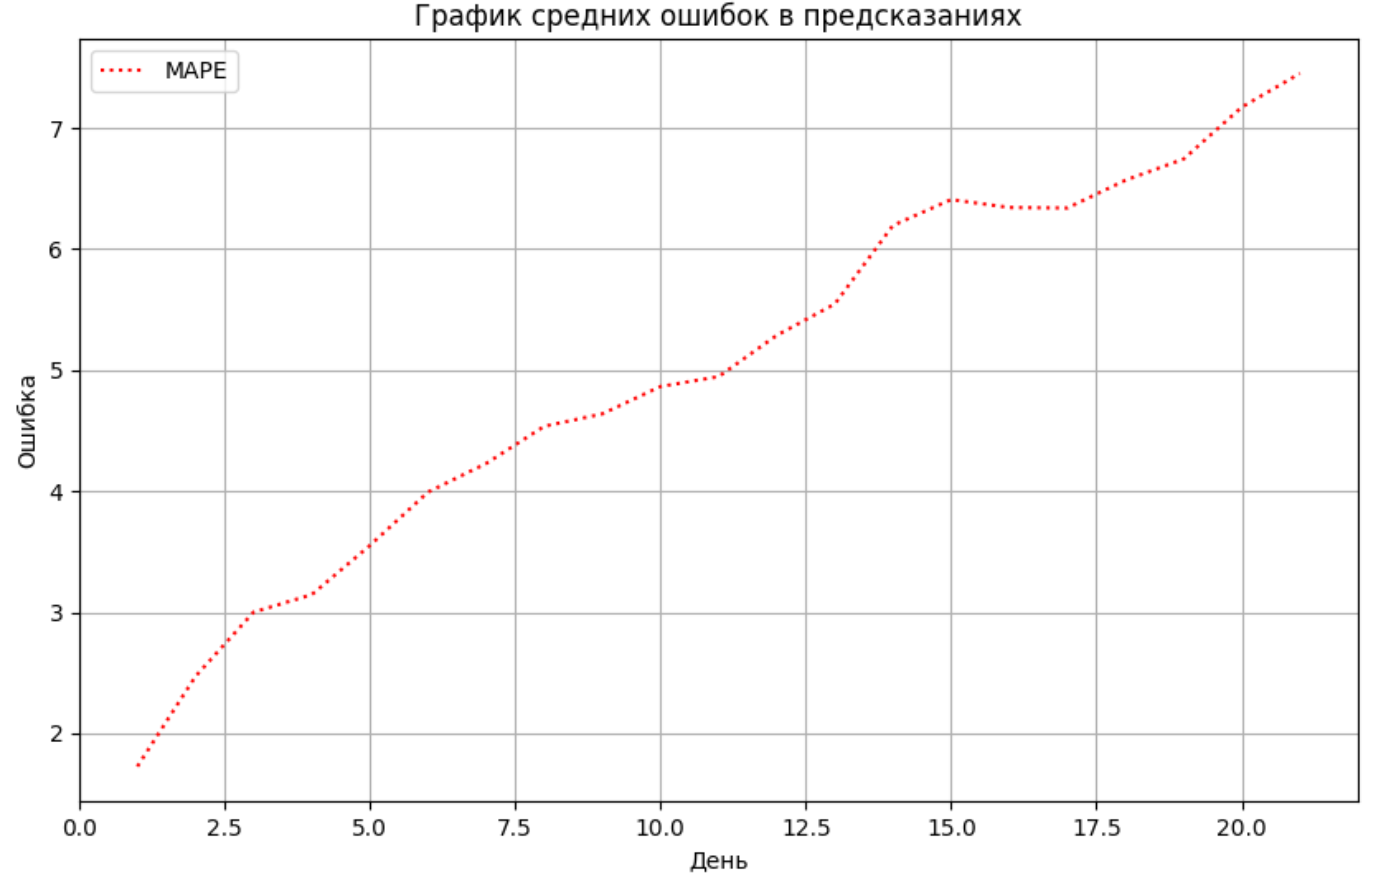
\includegraphics[width=1\linewidth]{xgboost}}
\caption{Средняя MAPE ошибка XGBRegressor на первый месяц.}
\label{fig:xgboost}
\end{figure}
\begin{figure}[H]
\center{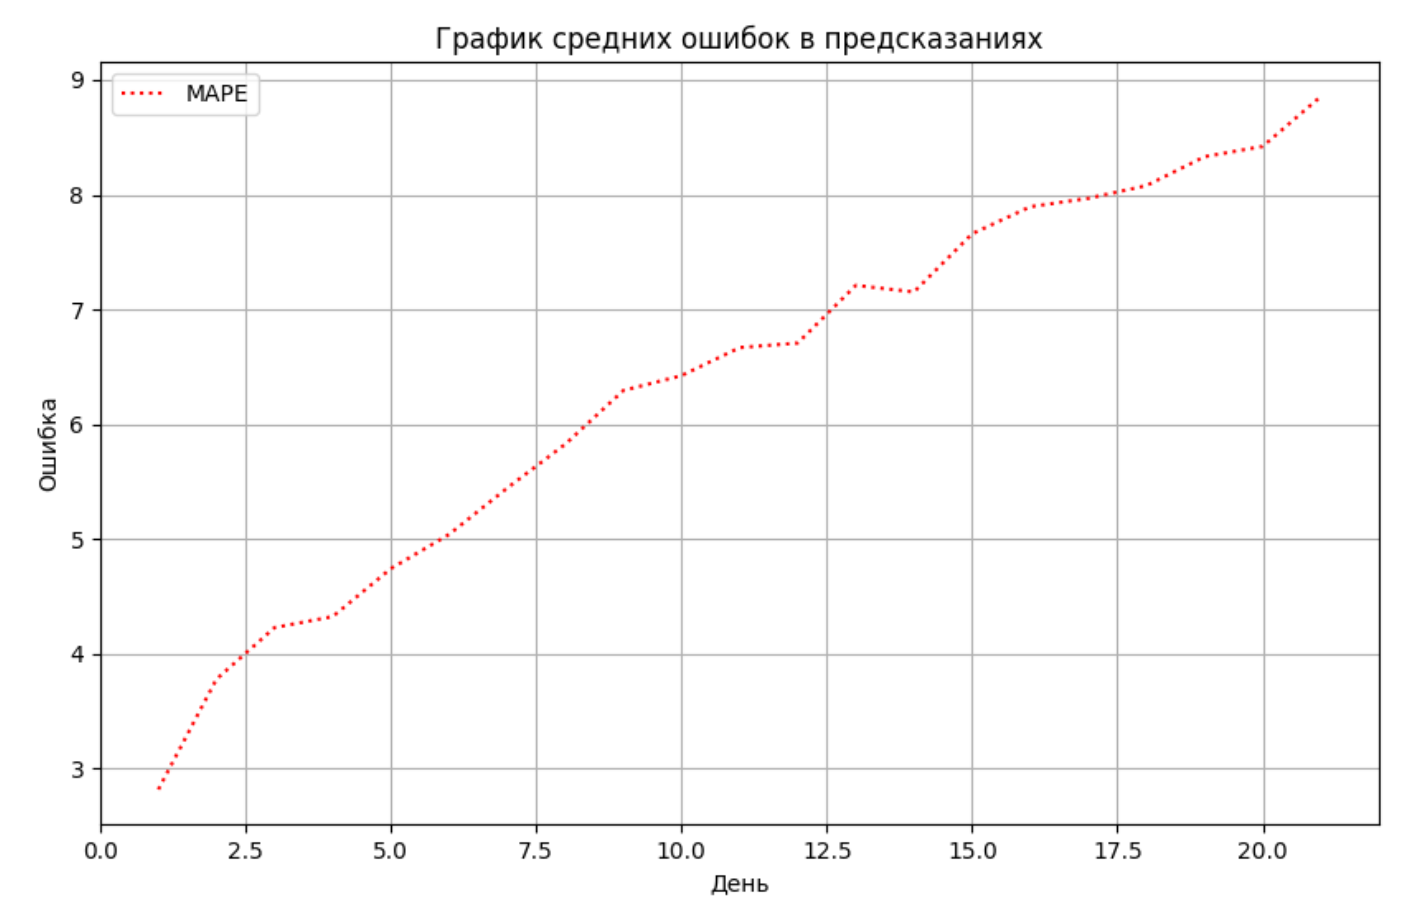
\includegraphics[width=1\linewidth]{xgboost_with_news}}
\caption{Средняя MAPE ошибка XGBRegressor с новостями на первый месяц.}
\label{fig:xgboost_with_news}
\end{figure}

\subsection{LSTM}

LSTM (Long Short-Term Memory) — это тип рекуррентной нейронной сети (RNN), предназначенный для обработки и предсказания последовательных данных. Вопрос касается принципов работы LSTM, его архитектуры и применения в задачах машинного обучения.

Основной подход был таким же, как и в предыдущих моделях, за исключением того, что вместо GridSearchCV я использовался Sequential.

Первый слой состоял из 48 нейронов с регуляризацией recurrent\_dropout=0.1,\\return\_sequences = True и инициализацией весов с помощью метода he\_normal. Затем следовал слой нормализации, и отключение 20\% нейронов. После чего шел второй слой LSTM с 24 нейронами и return\_sequences = False. Далее еще один слой нормализации и два полносвязных слоя: первый с функцией активации ReLU, а второй - с числом ожидаемых значений. Для обычной модели - единица (только стоимость), для модели с новостями - вывод девяти значений (стоимость и данные ожидаемых новостей).

Оптимизатор использовался Adam со скоростью обучения 0.001 и clipnorm=1.0. Функция потерь - Huber. Обратный вызов останавливается после 15 эпох, если валидационная ошибка не улучшается, восстанавливает лучшие веса. Также было использовано динамическое изменение скорости обучения: после 50 эпохи величина с каждым разом уменьшалась на 5\%.

К сожалению, данная модель показала себя хуже остальных, хотя средняя ошибка за две недели не изменялась больше чем на процент, что видно по \textquote{Таблице \ref{tab:lstm}}. На \textquote{Рисунке \ref{fig:lstm}} и \textquote{Рисунке \ref{fig:lstm_with_news}} видно, что средняя MAPE ошибка за месяц изменилась менее чем на два процента.
\begin{table}[h!]
\centering
\caption{Таблица средних ошибок LSTM на две недели.}
\begin{tabular}{ |c|c|c|c|c| } 
 \hline
 День предсказания & LSTM RMSE & LSTM + news RMSE & LSTM MAPE & LSTM + news MAPE \\ 
 \hline
1 & \textbf{179.778} & 358.869 & \textbf{12.284} & 19.643 \\ 
 \hline
2 & \textbf{176.325} & 352.127 & \textbf{12.432} & 20.080 \\ 
 \hline
3 & \textbf{194.466} & 347.170 & \textbf{12.219} & 20.286 \\ 
 \hline
4 & \textbf{193.421} & 357.515 & \textbf{12.000} & 19.972 \\ 
 \hline
5 & \textbf{190.941} & 353.370 & \textbf{12.091} & 20.026 \\ 
 \hline
6 & \textbf{193.543} & 350.417 & \textbf{12.283} & 20.106 \\ 
 \hline
7 & \textbf{204.219} & 351.025 & \textbf{12.167} & 20.019 \\ 
 \hline
8 & \textbf{216.102} & 373.916 & \textbf{12.117} & 20.152 \\ 
 \hline
9 & \textbf{220.227} & 376.465 & \textbf{12.148} & 20.440 \\ 
 \hline
10 & \textbf{214.584} & 380.385 & \textbf{12.237} & 20.377 \\ 
 \hline
\end{tabular}
\label{tab:lstm}
\end{table}
\begin{figure}[!h]
\center{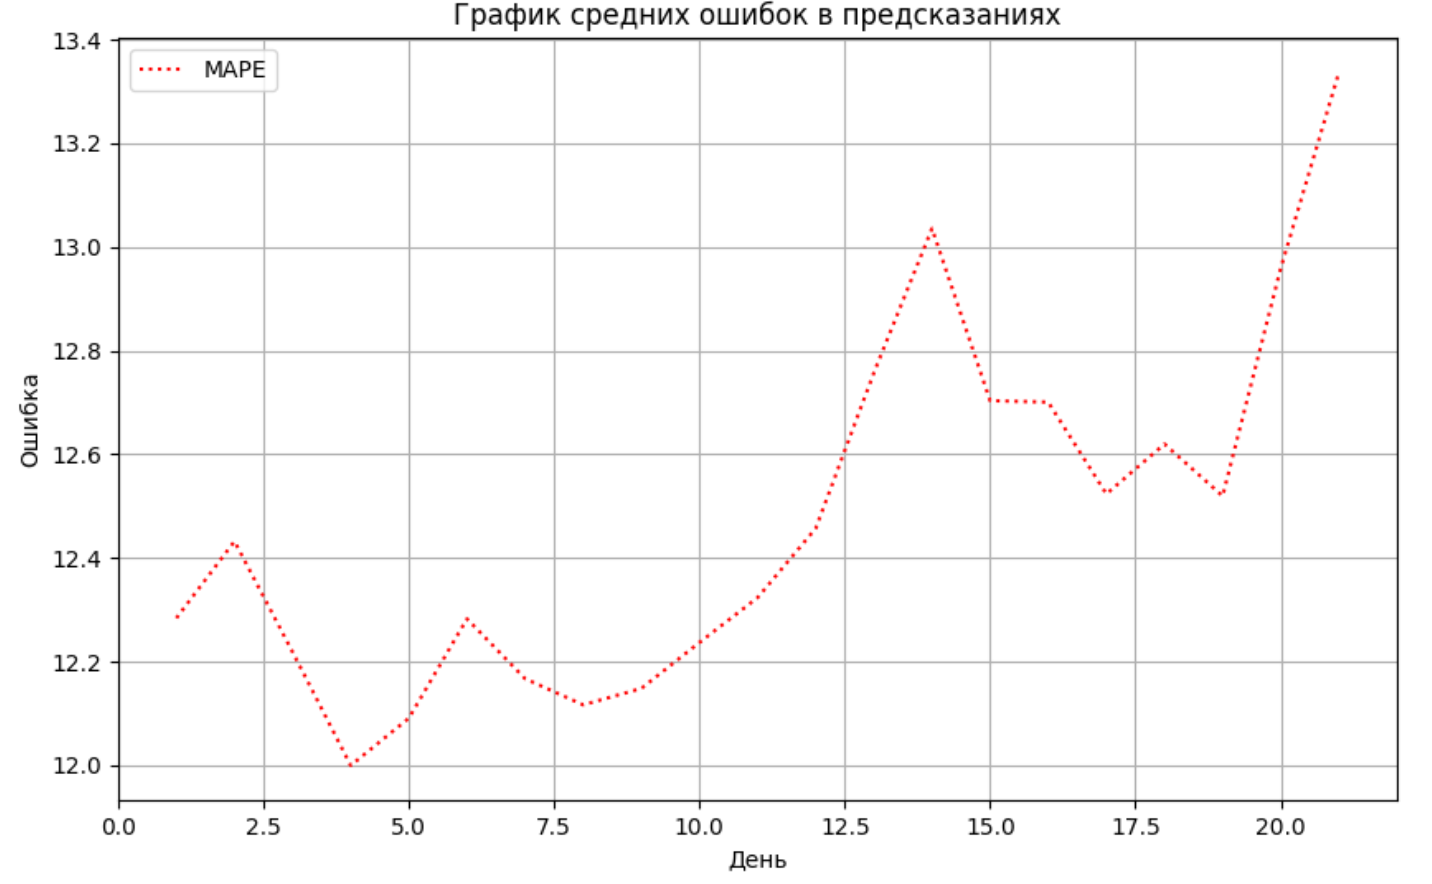
\includegraphics[width=1\linewidth]{lstm}}
\caption{Средняя MAPE ошибка LSTM на первый месяц.}
\label{fig:lstm}
\end{figure}
\begin{figure}[!h]
\center{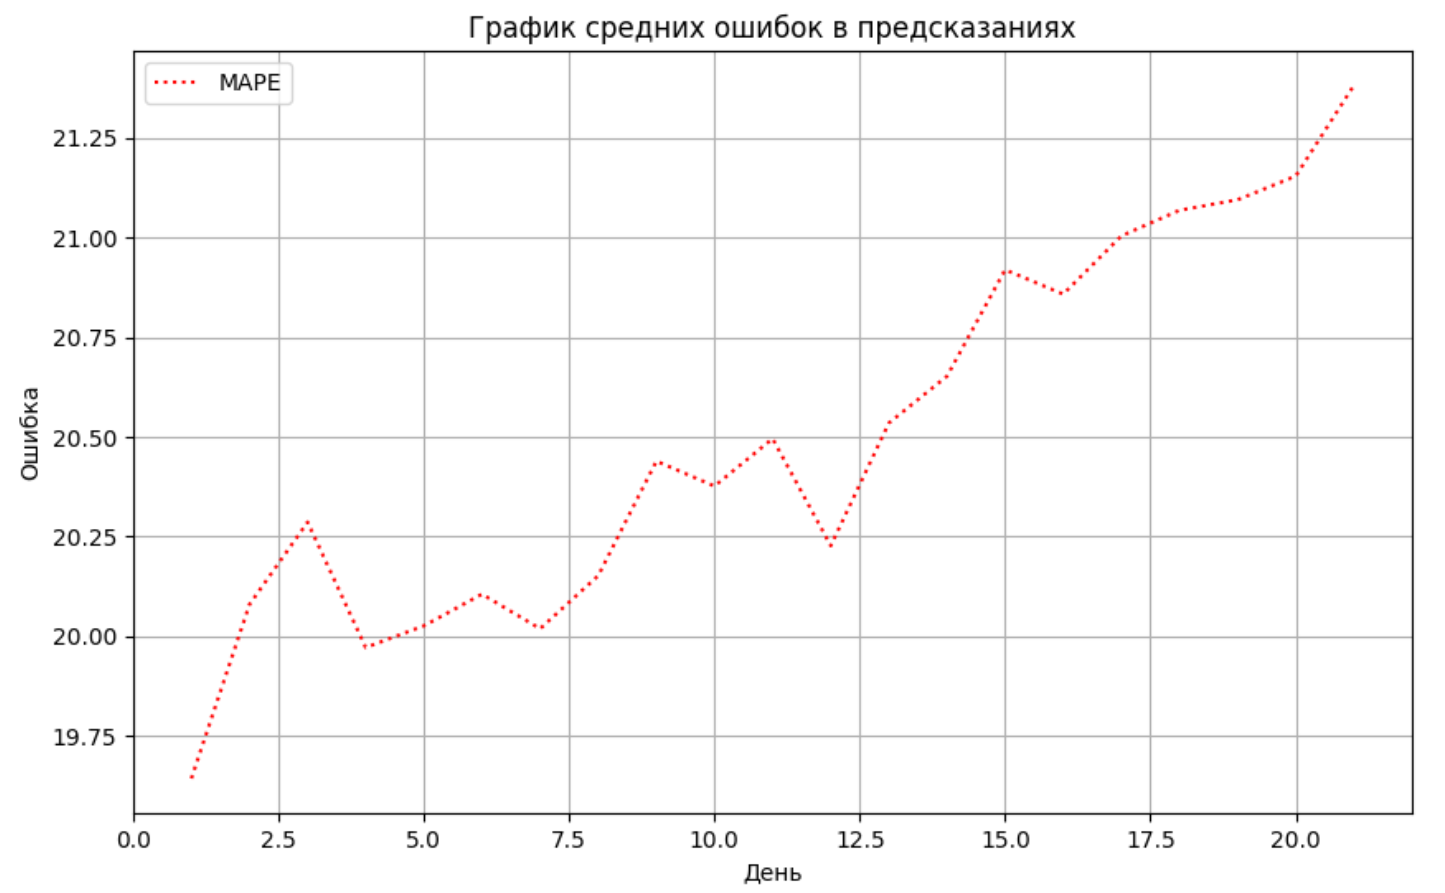
\includegraphics[width=1\linewidth]{lstm_with_news}}
\caption{Средняя MAPE ошибка LSTM с новостями на первый месяц.}
\label{fig:lstm_with_news}
\end{figure}

Не сомневаюсь, что результаты по данной модели могут быть лучше, но это требует более тщательного подхода и большего количества времени. Но, не смотря на такие средние результаты, данная модель и её версия с новостями часто оказываются в числе лучших для некоторых акций.

\subsection{Результаты исследований}

Итак, основная причина того, что модели с новостями в среднем показывают результат хуже, чем без них. Я считаю, что это связано с тем, что сами новости в полном объёме для каждой из компаний сложно получить. Я пробовал для каждой новости получить все возможные влияния на каждую из бумаг, что не так просто. Но еще сложнее получить новости по менее популярным акциям. Это я к тому, что условный Сбер или Яндекс будут гораздо чаще фигурировать в новостных сводках, и влияние на их бизнес найти проще, чем на какую-то не столь большую компанию. Таким образом получается, что в модели число признаков становится слишком большим по отношению к числу данных, а их влияние практически невидимо из-за сложного выявления новостной информации.

Не вижу смысла рассматривать конкретные бумаги, потому что сутью было выявить лучшие модели, но, чтобы не сложилось мнение, что lstm плох или что новости не вносят важные данные, я бы привел в пример данные по тикеру ALRS.

Для неё лучшими моделями по MAPE были следующие: на первый день Random Forest с новостями и ошибкой 0.964\%, на пятый день SARIMAX с 0.1\%, десятый (две недели), двадцать первый (месяц) и шестьдесят второй (квартал) дни в лидерах был LSTM с новостями с соответствующими процентами по MAPE 0.795, 0.403 и 2.026. На 124 (полгода) день в лидерах был Ridge с новостями с ошибкой 3.381, и через 247 дней (год) снова LSTM с новостями и ошибкой по MAPE 11.859.

На данном примере можно видеть, что в некоторых случаях, на некоторых бумагах, модели с новостями работают лучше, хотя в среднем результат у новостных моделей гораздо хуже. Также видно, что LSTM с новостями, показавшая худшие средние результаты, для данной бумаги на большем горизонте оказалась лучшей. Здесь была бумага эмитента Алроса, которая является достаточно крупной и известной в России, что помогло получить достаточно новостных данных для хорошего обучения и прогнозирования.

И в завершение этой главы я бы хотел по \textquote{Таблице \ref{tab:mean_results}} продемонстрировать, какие места в среднем на разных горизонтах времени занимала каждая из моделей. Как видно, в среднем лучшей оказывалась модель Random Forest, от которой почти всегда слегка отставала XGBRegressor. Если смотреть среди новостных моделей, то фаворитом определенно была модель XGBRegressor. 
\begin{table}[H]
\centering
\caption{Таблица средних мест моделей на горизонты дней.}
\begin{tabular}{ |c|c|c|c|c|c|c|c|c|c| } 
 \hline
День & SARIMAX & Ridge & Ridge+ & Forest & Forest+ & XGB & XGB+ & LSTM & LSTM+ \\ 
 \hline
1 & 4.78 & \textbf{3.27} & 3.85 & 3.73 & 5.33 & 4.06 & 4.47 & 7.37 & 8.14 \\ 
 \hline
5 & 5.28 & 4.01 & 4.72 & \textbf{3.70} & 5.14 & 4.06 & 4.24 & 6.35 & 7.50 \\
 \hline
10 & 5.59 & 4.12 & 4.53 & 3.92 & 5.21 & \textbf{3.83} & 4.42 & 6.02 & 7.36 \\
 \hline
21 & 7.01 & 4.15 & 4.38 & \textbf{3.86} & 4.95 & 3.94 & 4.45 & 5.34 & 6.93 \\
 \hline
62 & 8.15 & 3.99 & 4.88 & \textbf{3.78} & 5.01 & 3.81 & 4.39 & 4.55 & 6.44 \\
 \hline
124 & 8.73 & 4.14 & 4.60 & \textbf{3.65} & 4.95 & 3.68 & 4.04 & 4.24 & 6.01 \\
 \hline
247 & 8.08 & 4.45 & 4.62 & \textbf{3.14} & 4.26 & 4.06 & 3.95 & 3.76 & 5.35 \\
 \hline
\end{tabular}
\label{tab:mean_results}
\end{table}

Рассмотрев все вышеописанные модели и полученные результаты, я бы сказал, что в общем случае лучше выбирать Random Forest Regression модель, она достаточно хороша в начале и отлично работает на большем периоде. Лучше неё может быть модель Ridge Regression, но только на коротком промежутке. Ну и если новостей по бумаге много, эмитент обсуждаемый или популярный, но не только ставший таким заметным, то можно попробовать XGBRegressor с новостями. Также имеет смысл использовать LSTM, но для работы с ним необходимо потратить много времени и сил. Ну а ARIMA-подобные модели я бы не рекомендовал, для биржевого рынка лучше иметь больше факторов, а данное семейство моделей не очень подходит.

\section{Сервис}
\subsection{Архитектура}

Не менее важен сервис. Для написания серверной части я выбрал Python-фреймворк FastAPI. Для большего удобства пользователям в качестве визуального представления клиентам я выбрал Streamlit. В качестве базы данных я решил не отходить от облачного хранилища Яндекс S3. Для придания более серьезного вида мною были добавлены Nginx и SSL-сертификат. А для большего удобства развертывания использовал Docker Compose.

FastAPI — это современный веб-фреймворк для создания API на Python, который позволяет разработчикам быстро и эффективно разрабатывать приложения. Он основан на стандартных Python-типах и использует асинхронные функции, что обеспечивает высокую производительность.

Streamlit — это фреймворк с открытым исходным кодом, который позволяет разработчикам создавать веб-приложения для визуализации данных и взаимодействия с моделями машинного обучения. Он был разработан с целью упростить процесс создания приложений, позволяя сосредоточиться на логике и визуализации, а не на сложностях веб-разработки.

S3-хранилище Яндекс — это облачное решение для хранения и управления данными, которое предоставляет пользователям возможность хранить неструктурированные данные, такие как изображения, видео, резервные копии и другие файлы. Оно основано на принципах, схожих с Amazon S3, и предлагает высокую доступность, масштабируемость и безопасность.

Nginx — это мощный веб-сервер, который также может выполнять функции балансировщика нагрузки. Он позволяет распределять входящий трафик между несколькими серверами, что обеспечивает высокую доступность и масштабируемость приложений.

SSL (Secure Sockets Layer) сертификат — это цифровой сертификат, который подтверждает личность веб-сайта и шифрует данные, передаваемые между пользователем и сервером. Он обеспечивает защиту от перехвата данных и атак типа "человек посередине".

Docker Compose — это инструмент, который позволяет определять и запускать многоконтейнерные приложения Docker. Он использует файл конфигурации в формате YAML для описания сервисов, сетей и томов, необходимых для работы приложения.

Таким образом, получается следующая схема. Поднимается сервер с использованием Docker Compose, после чего становятся доступны FastAPI и Streamlit, на которые клиент может делать запросы. Далее Nginx перехватывает запросы и решает, куда их направить. После получения запроса на Streamlit от клиента идёт обращение на бэкенд. Далее FastAPI ищет информацию в своей памяти или делает запрос к S3 Яндекс. Получив от облачного хранилища данные по запросу, FastAPI их обрабатывает и возвращает данные в Streamlit или клиенту. В случае, если клиент делал запрос не напрямую на бэкенд, то полученный ответ Streamlit обрабатывает и отдаёт в удобном для понимания виде, после чего снова ожидается запрос от клиента.
\begin{figure}[!h]
\center{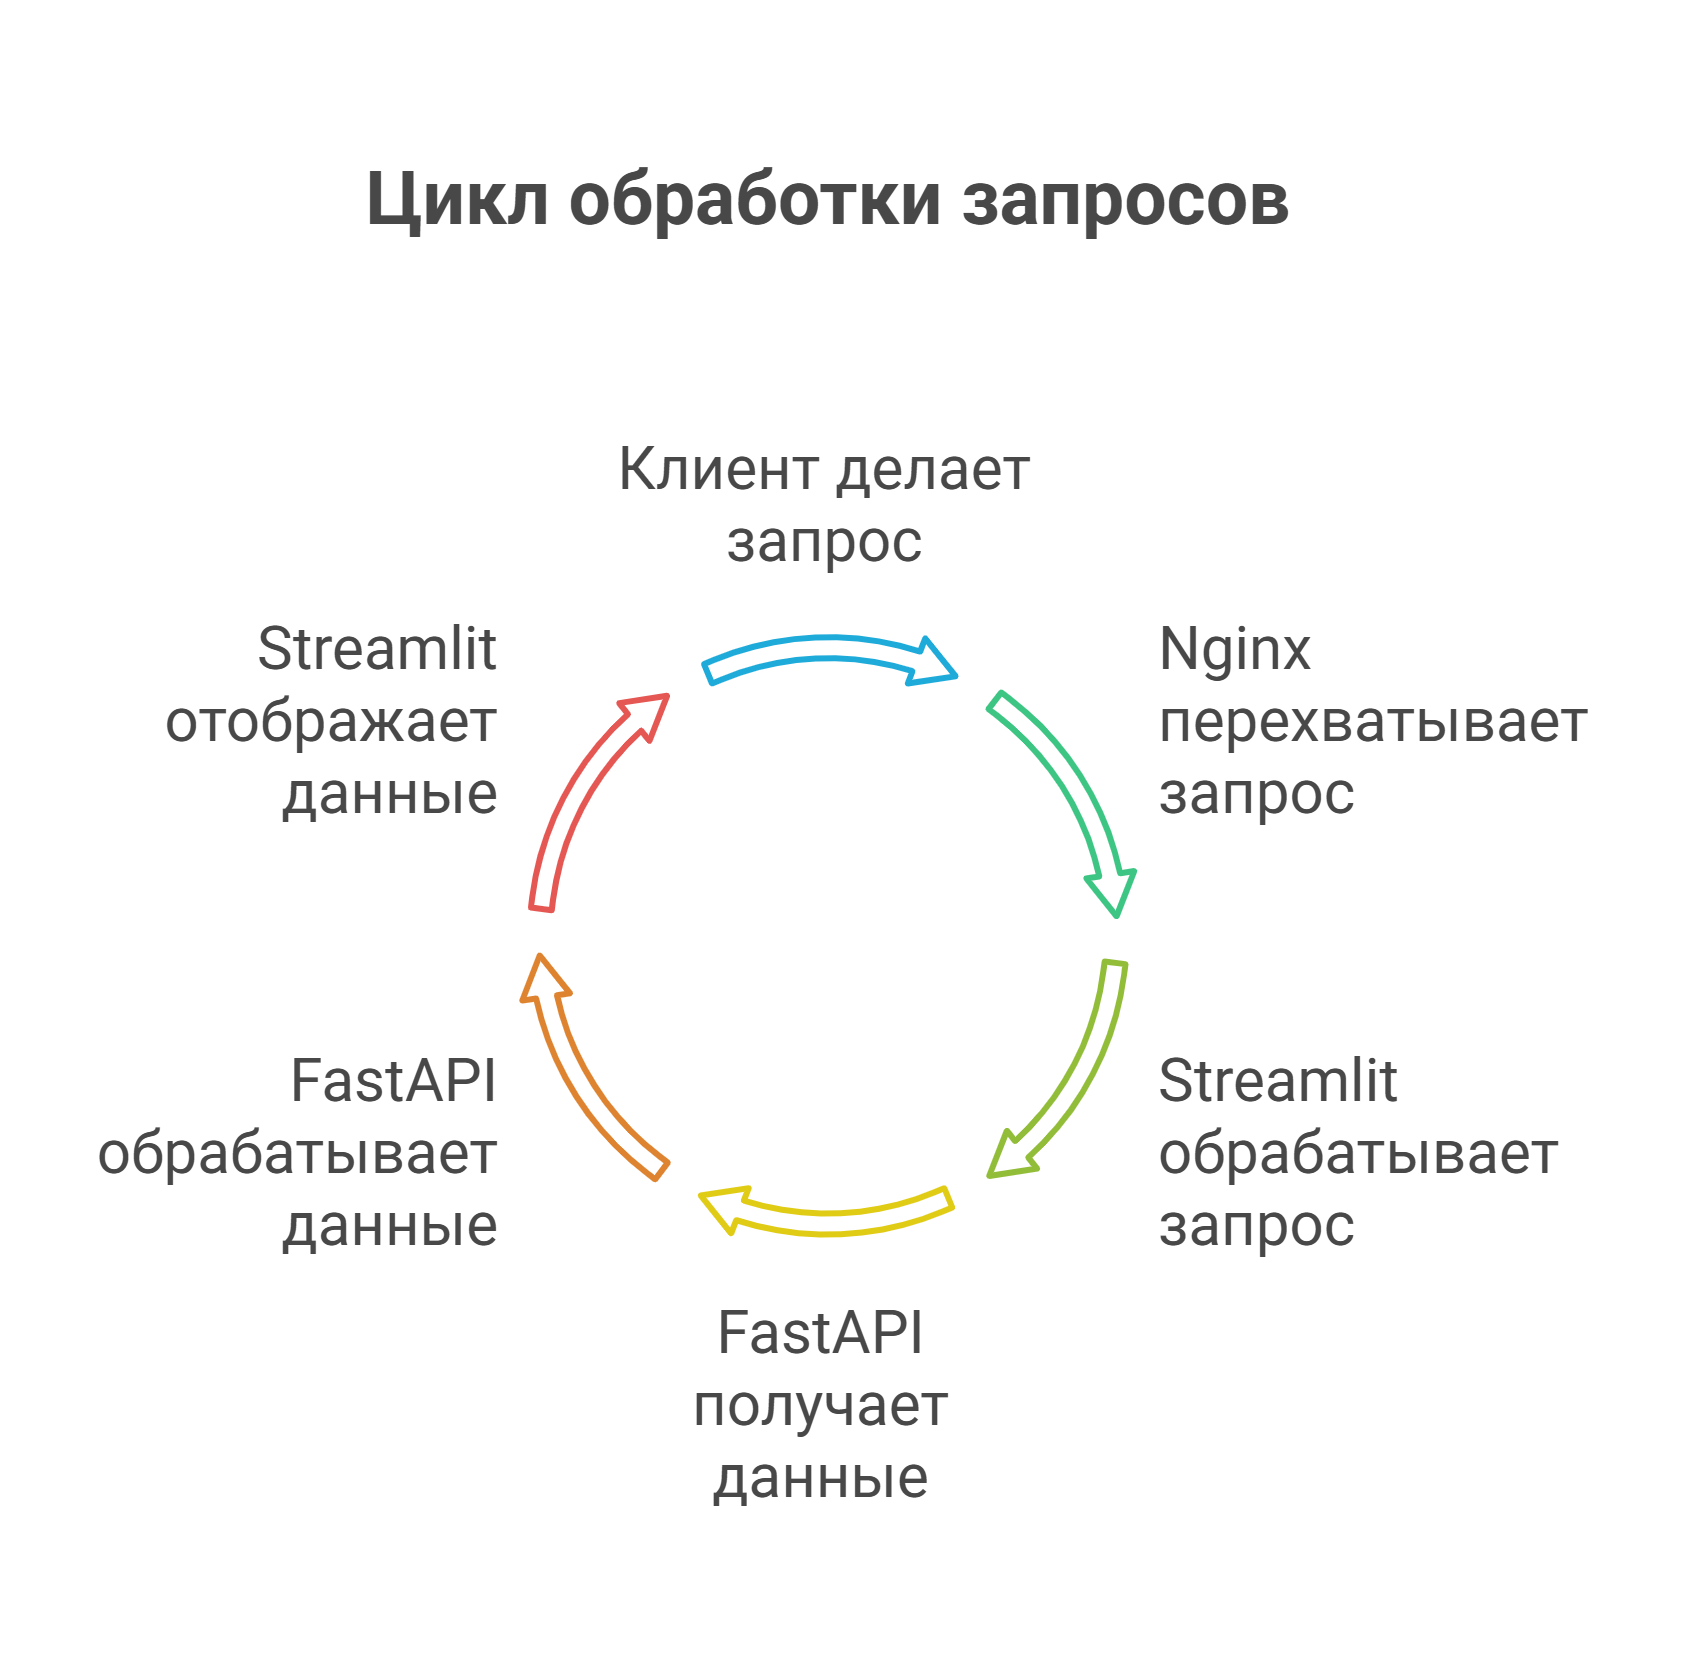
\includegraphics[width=1\linewidth]{service}}
\caption{Цикл обработки запросов.}
\label{fig:service}
\end{figure}

\subsection{Запросы API}

Достыпные запросы описаны в \textquote{Таблице \ref{tab:api_requests}}. И на \textquote{Рисунке \ref{fig:api_endpoints}}

\begin{table}[h!]
\centering
\caption{Содержание запросов.}
\begin{tabular}{ |c|c|c|c| } 
 \hline
Запрос & Суть запроса & Принимает & Возвращает \\ 
 \hline
/secids/ & Получение тикеров компаний & - & Список доступных тикеров \\ 
 \hline
/models/ & Получение моделей & - & Список обученных моделей \\ 
 \hline
\shortstack{/predict/\{model\}/\\\{secid\}/} & \shortstack{Получение данных\\для конкретного\\тикера и модели} & \shortstack{Тикер акции,\\ модель} & \shortstack{Прогноз цен акции,\\ошибки на каждый день,\\данные для\\соответствующих графиков} \\ 
 \hline
\shortstack{/predict\_mean/\\\{model\}/\{secid\}/} & \shortstack{Получение среднего графика\\для определенной модели\\на всех тикерах\\или старше пяти лет} & \shortstack{Модель, горизонт} & \shortstack{Прогноз средних ошибок\\на каждый день,\\данные для\\соответствующих графиков} \\ 
 \hline
\shortstack{/top\_models/\\\{duration\}/} & \shortstack{Среднее занимаемое\\место моделью в\\качестве прогнозов} & \shortstack{Горизонт} & \shortstack{Данные для графиков\\средних мест моделей\\на разные горизонты} \\ 
 \hline
\end{tabular}
\label{tab:api_requests}
\end{table}
\begin{figure}[!h]
\center{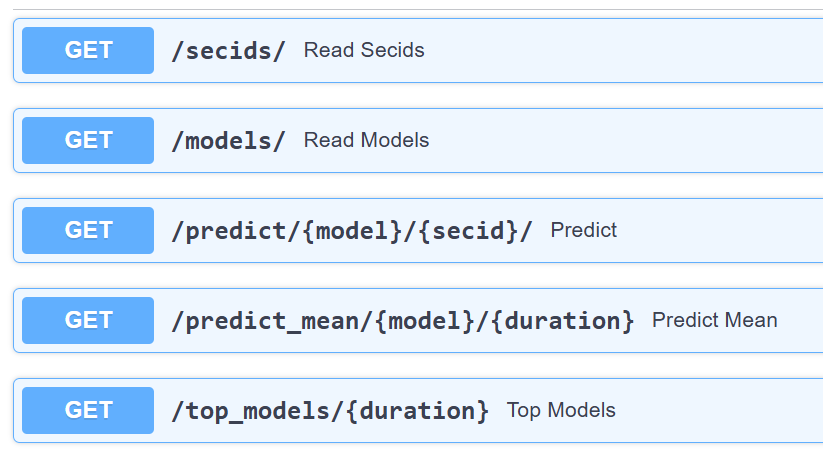
\includegraphics[width=1\linewidth]{api_endpoints}}
\caption{Доступные endpoint'ы.}
\label{fig:api_endpoints}
\end{figure}

\subsection{Общая структура сервиса}

Сервис представлен тремя страницами:

\begin{itemize}
  \item Акции - страница позволяет выбрать акцию и модель, а также посмотреть прогнозы и оценить их точность.
  \item Среднее - на этой странице можно увидеть, насколько хорошо та или иная модель справляется с предсказаниями и какие в среднем ошибки она имеет.
  \item Топ моделей - страница предоставляет информацию о местах, которые каждая из моделей занимает на разных горизонтах для множества доступных акций.
\end{itemize}

Каждая страница состоит из двух областей: левой боковой панели
(сайдбара) с настройками и основной области, в которой происходит
визуализация результатов.

\subsection{Функионал}

На странице с акциями можно выбрать тикер и модель, после чего, как на \textquote{Рисунке \ref{fig:stocks}} будет отображена таблица с прогнозами и ошибками, график цен, а также графики валидации с прогнозом и ошибки по периодам, как на \textquote{Рисунке \ref{fig:stocks_other}}.
\begin{figure}[!h]
\center{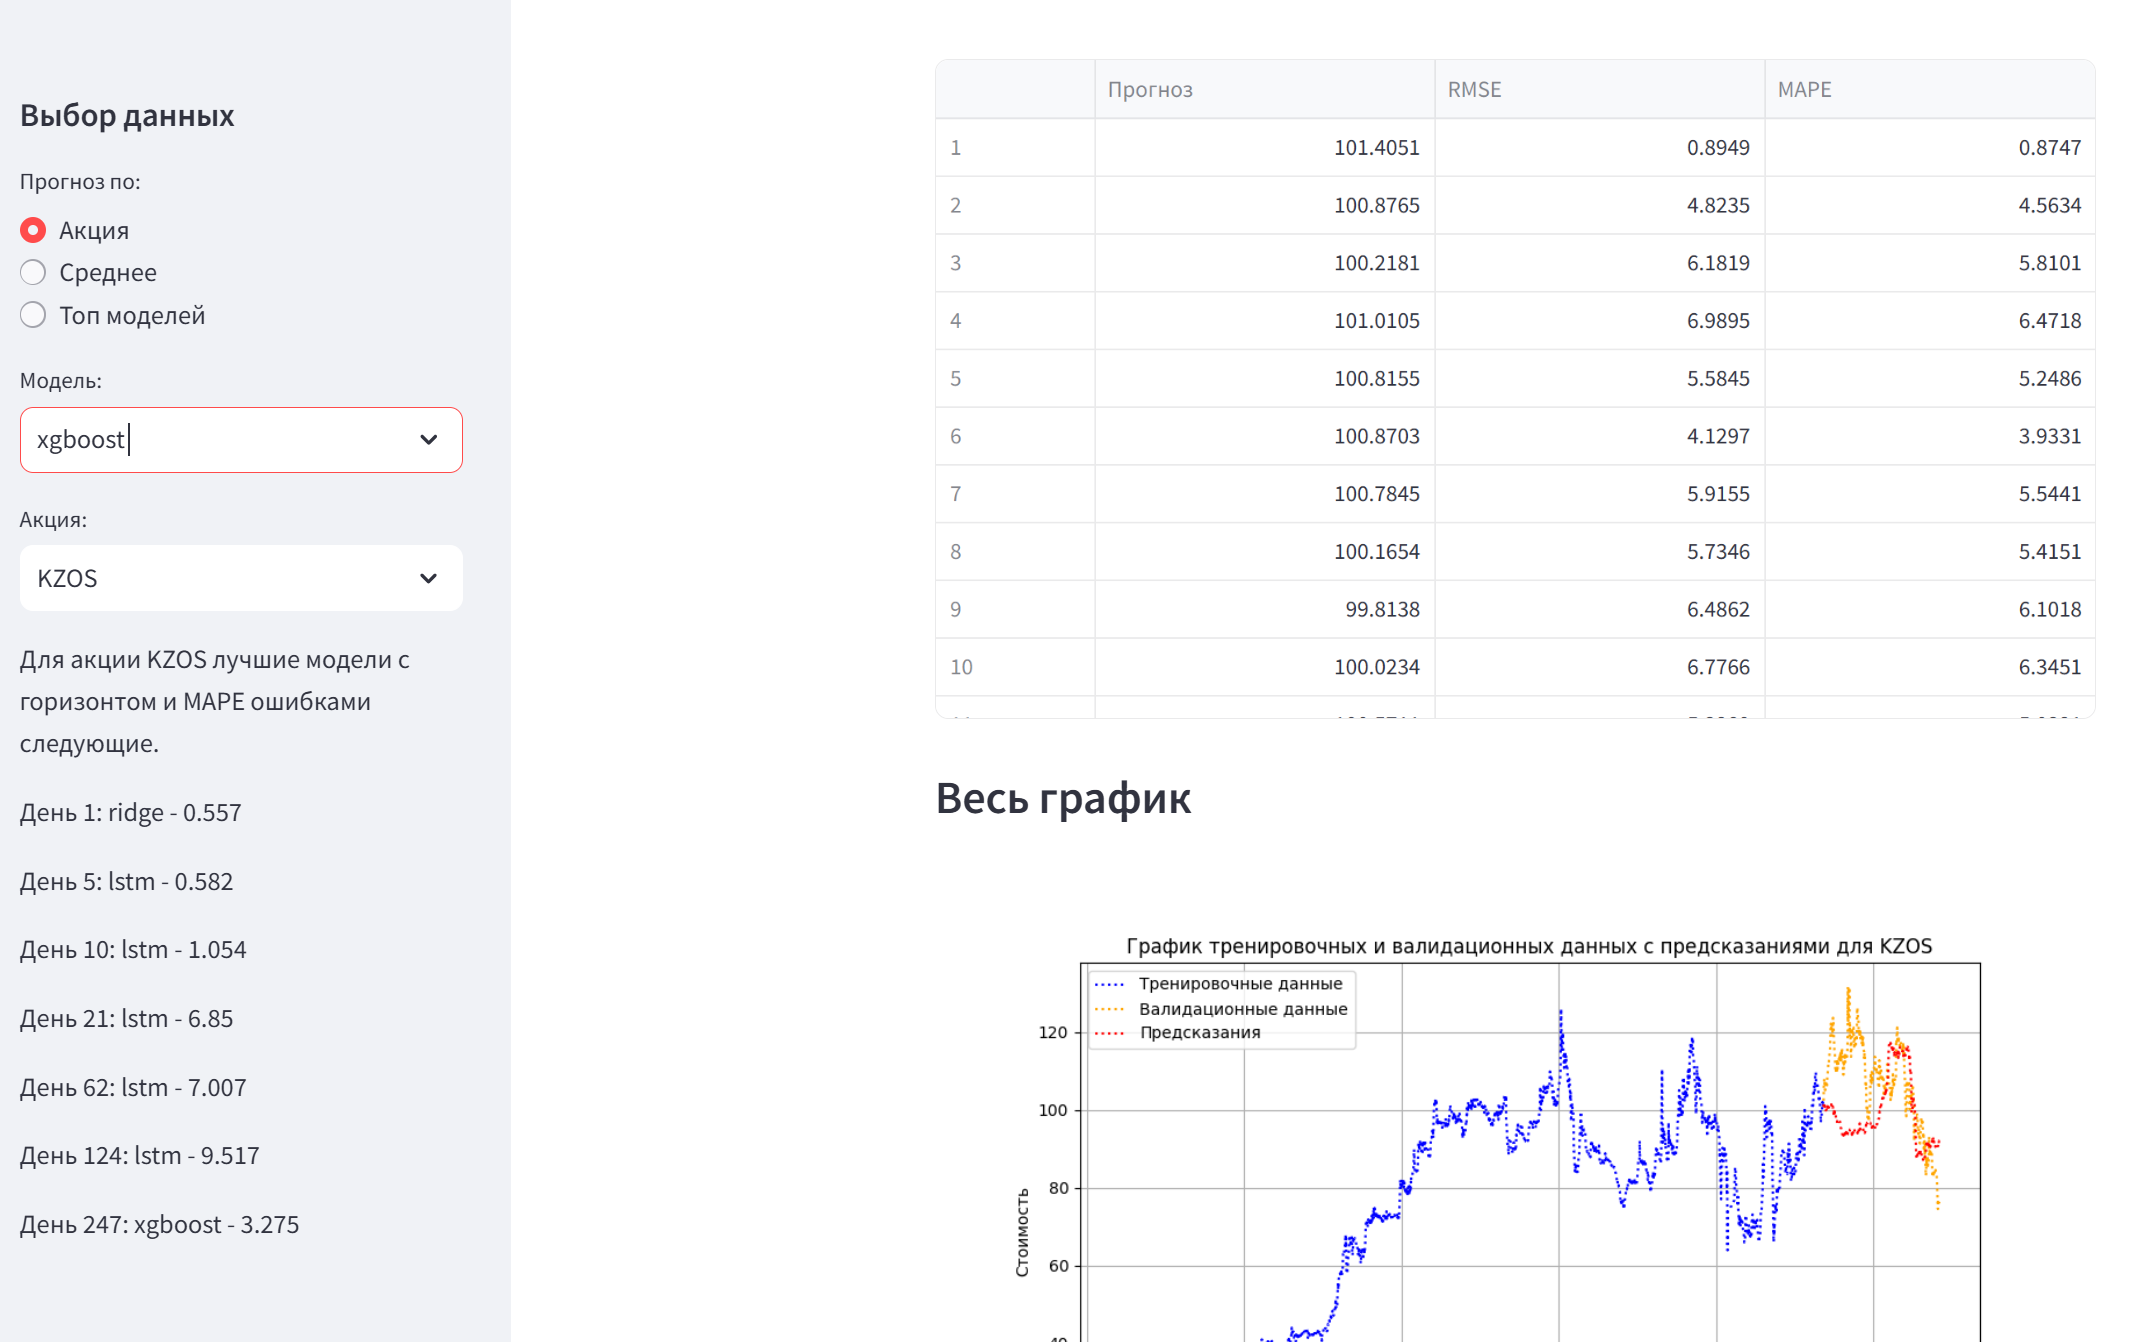
\includegraphics[width=1\linewidth]{stocks}}
\caption{Страница акций: основные данные.}
\label{fig:stocks}
\end{figure}
\begin{figure}[!h]
\center{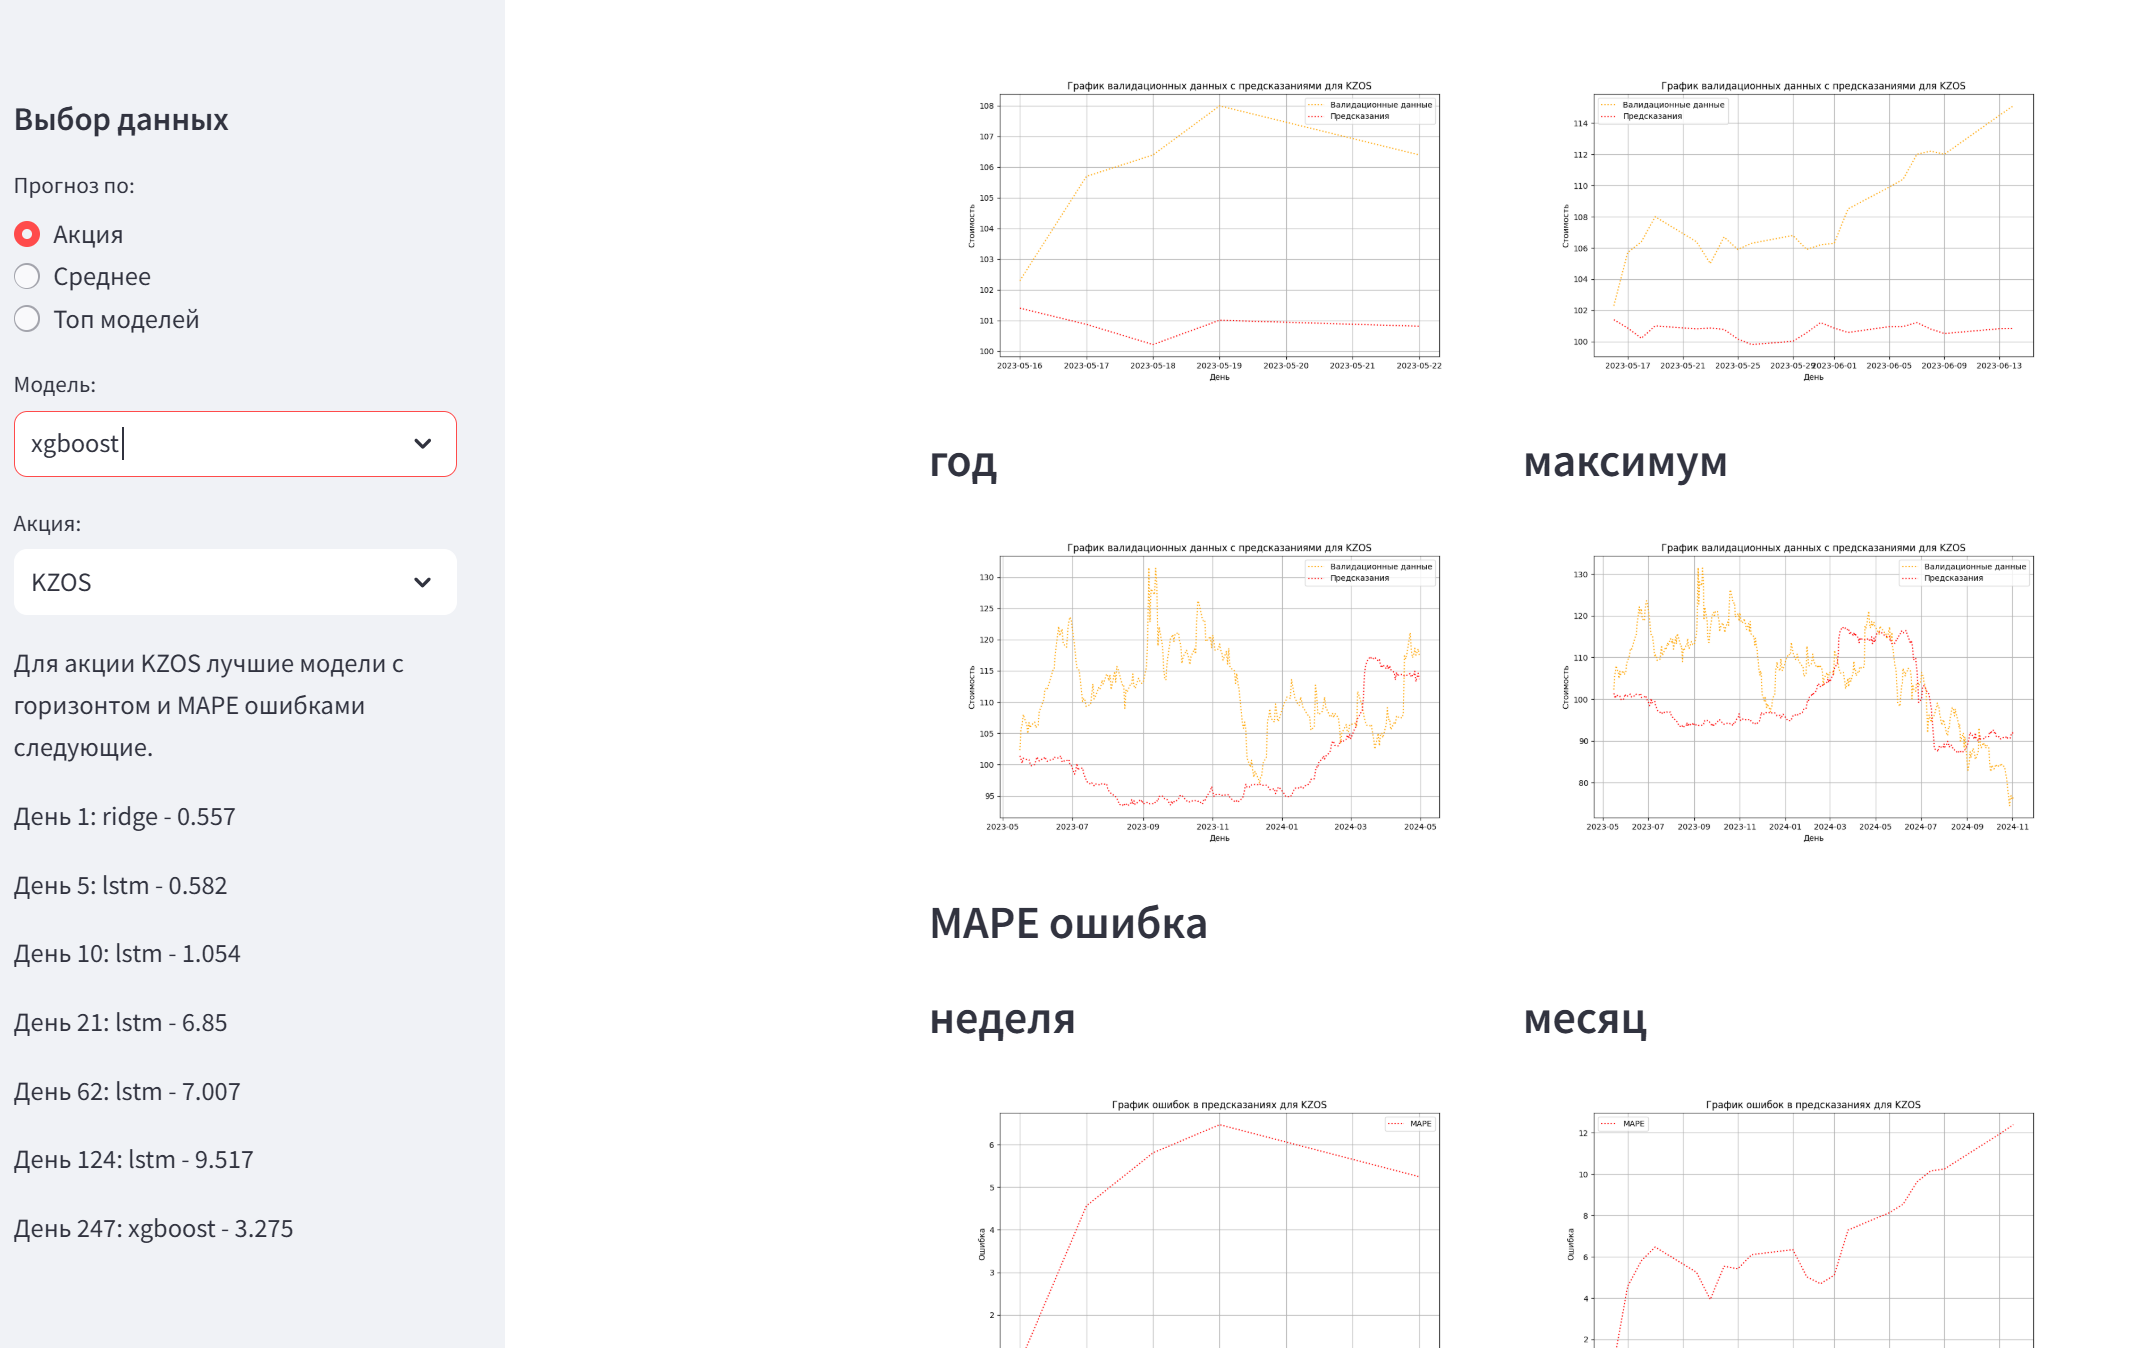
\includegraphics[width=1\linewidth]{stocks_other}}
\caption{Страница акций: данные с удобными отрезками.}
\label{fig:stocks_other}
\end{figure}

Для большего удобства слева продемонстрировано, на каких горизонтах какая модель для данной бумаги оказалась точнее.

Страница со средними результатами показывает полученные средний данные модели на множестве акций. На \textquote{Рисунке \ref{fig:mean}} видна таблица со средними ошибками и соответствующие графики, дополненные на \textquote{Рисунке \ref{fig:mean_other}}.
\begin{figure}[!h]
\center{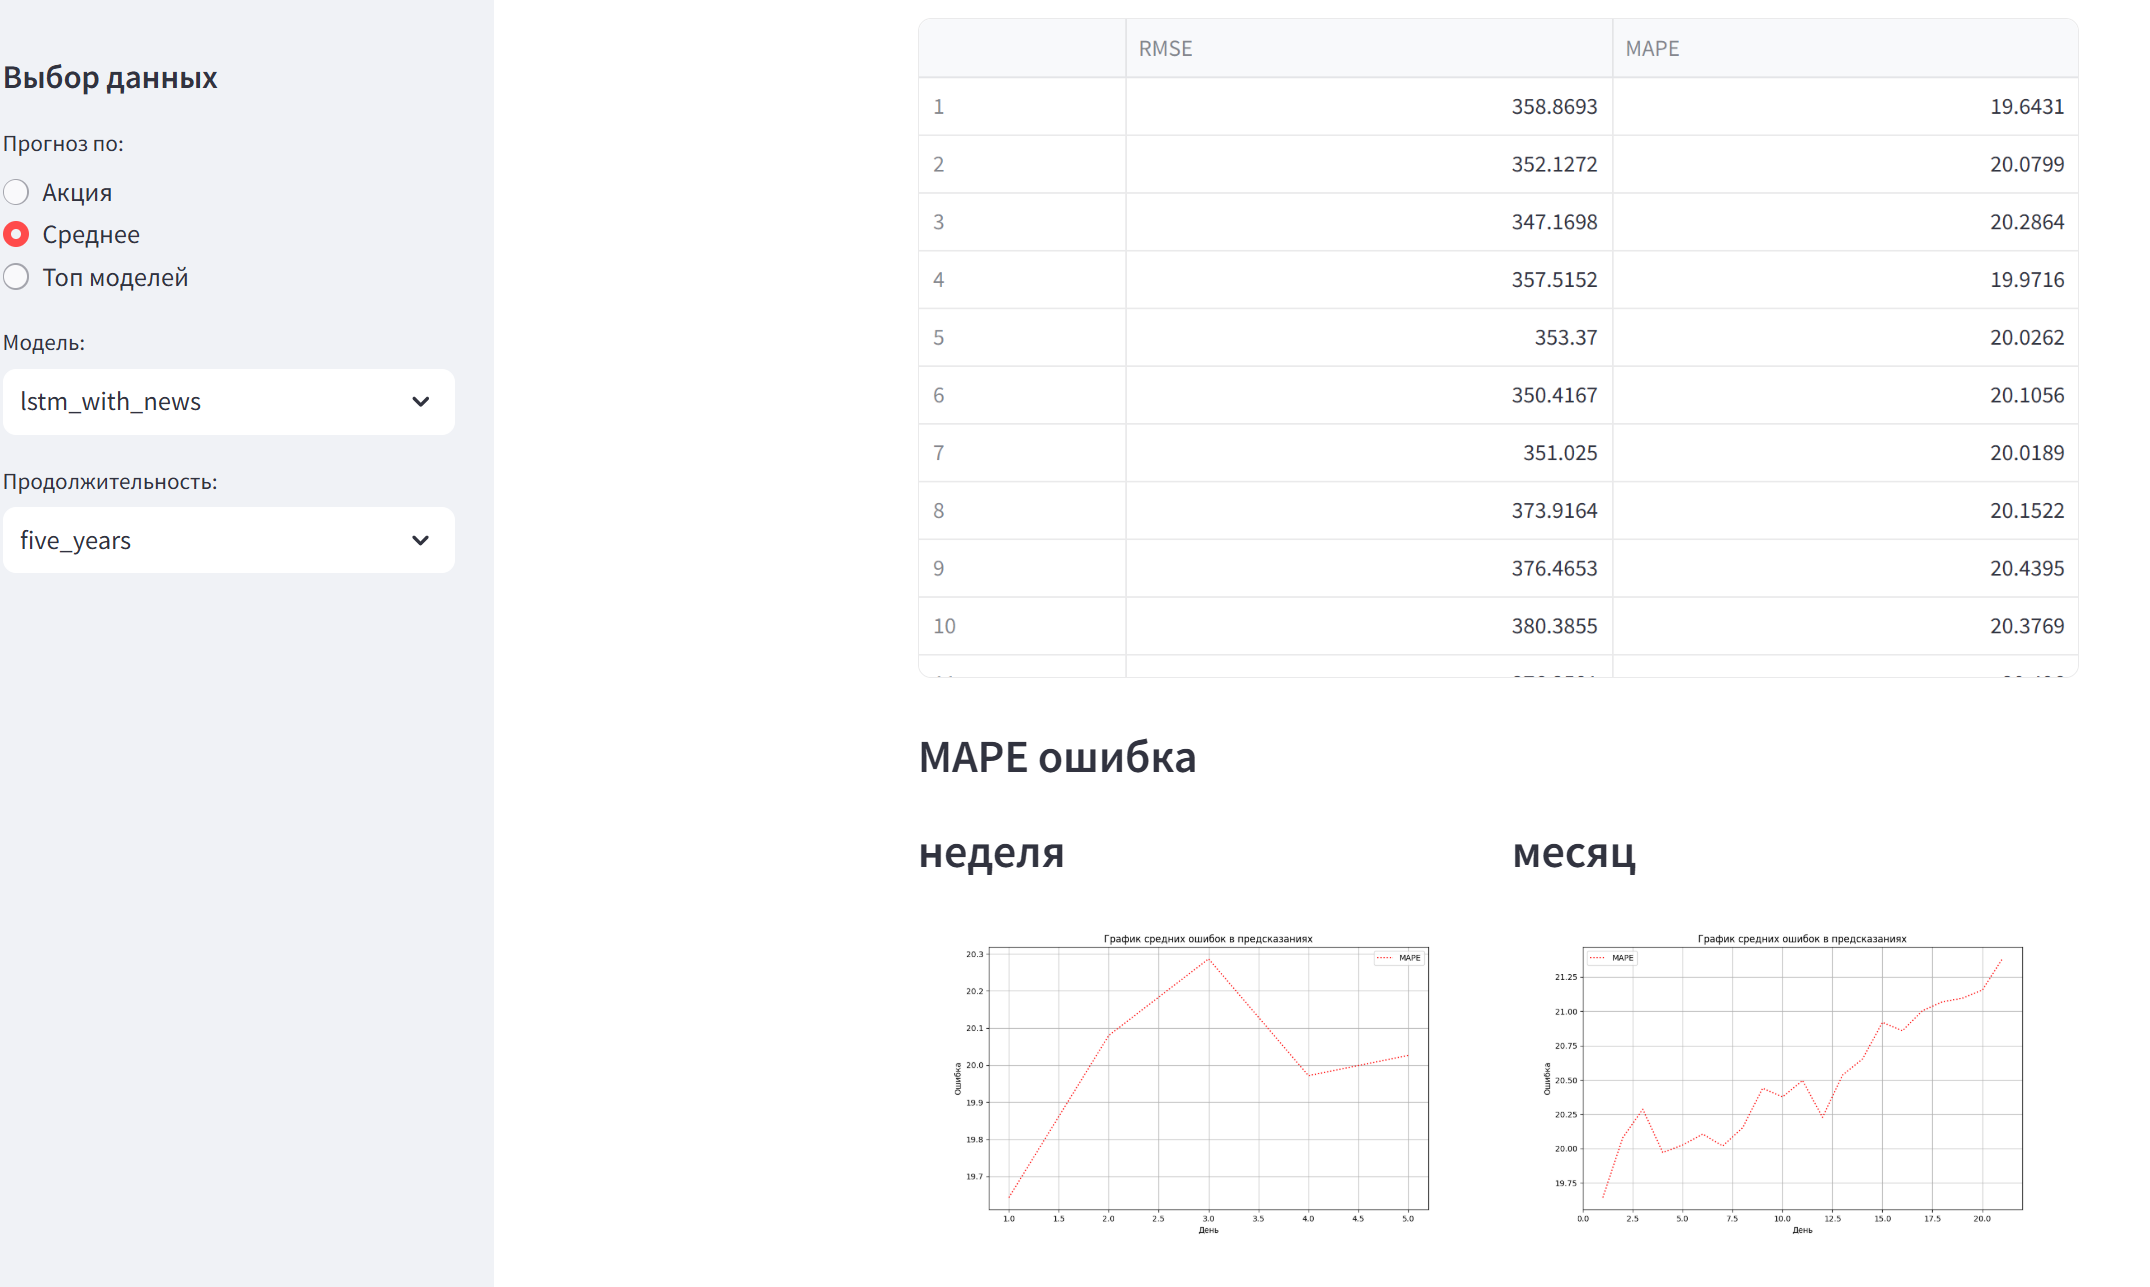
\includegraphics[width=1\linewidth]{mean}}
\caption{Страница средних данных по модели.}
\label{fig:mean}
\end{figure}
\begin{figure}[!h]
\center{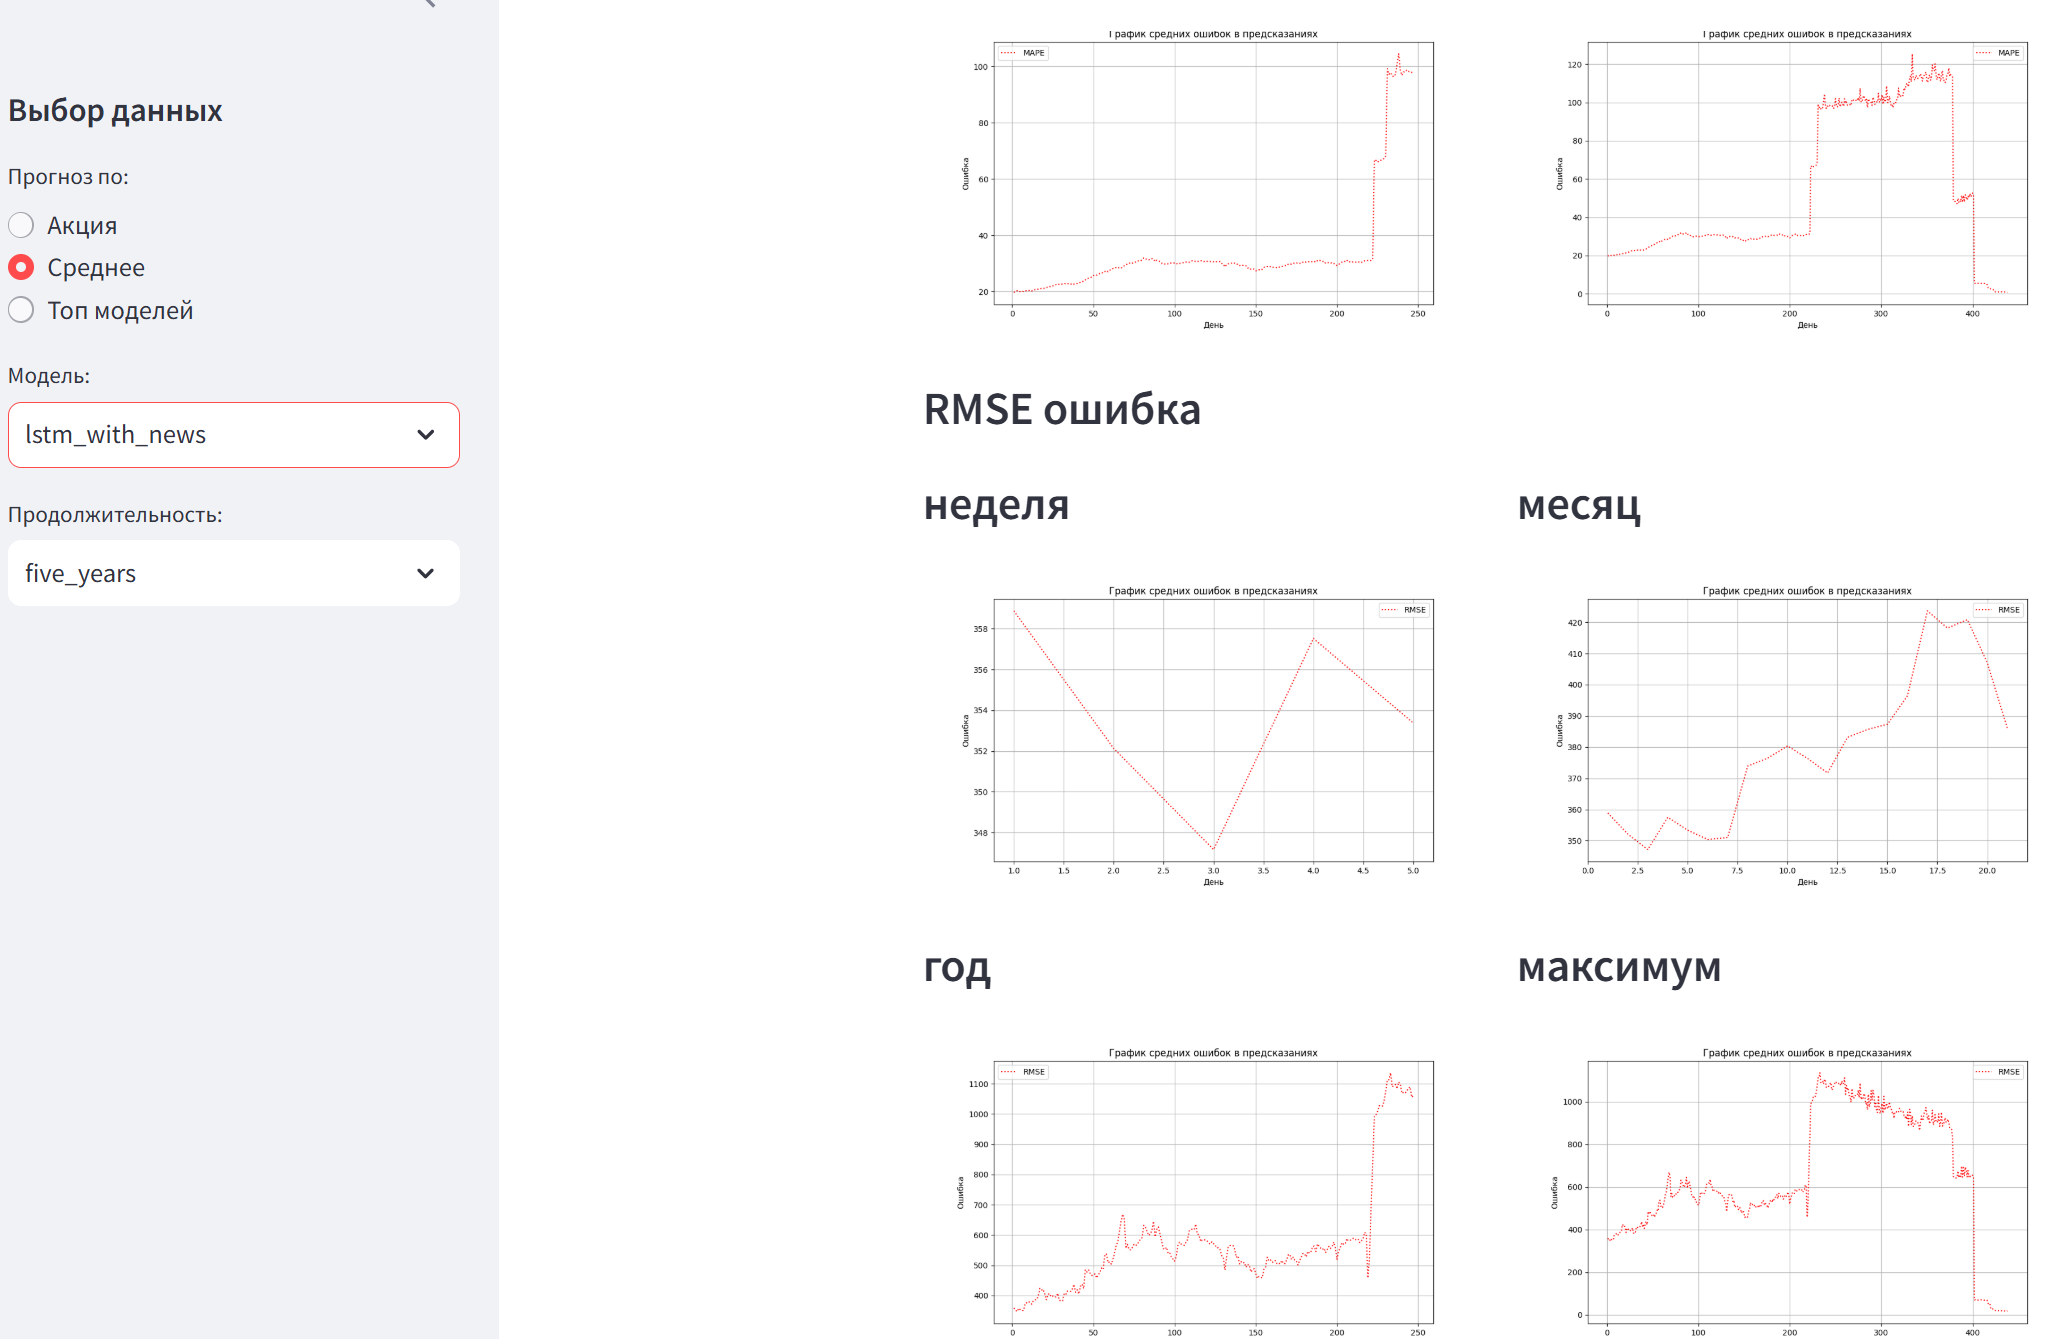
\includegraphics[width=1\linewidth]{mean_other}}
\caption{Страница графиков средних данных по модели.}
\label{fig:mean_other}
\end{figure}

И последняя страница рассказывает о том, какая модель на каком горизонте в среднем лучше показывала свои результаты, то есть как часто она занимала лучшие места. На \textquote{Рисунке \ref{fig:top}} и \textquote{Рисунке \ref{fig:top_other}}, видны лидеры и то, как они меняются со временем.
\begin{figure}[H]
\center{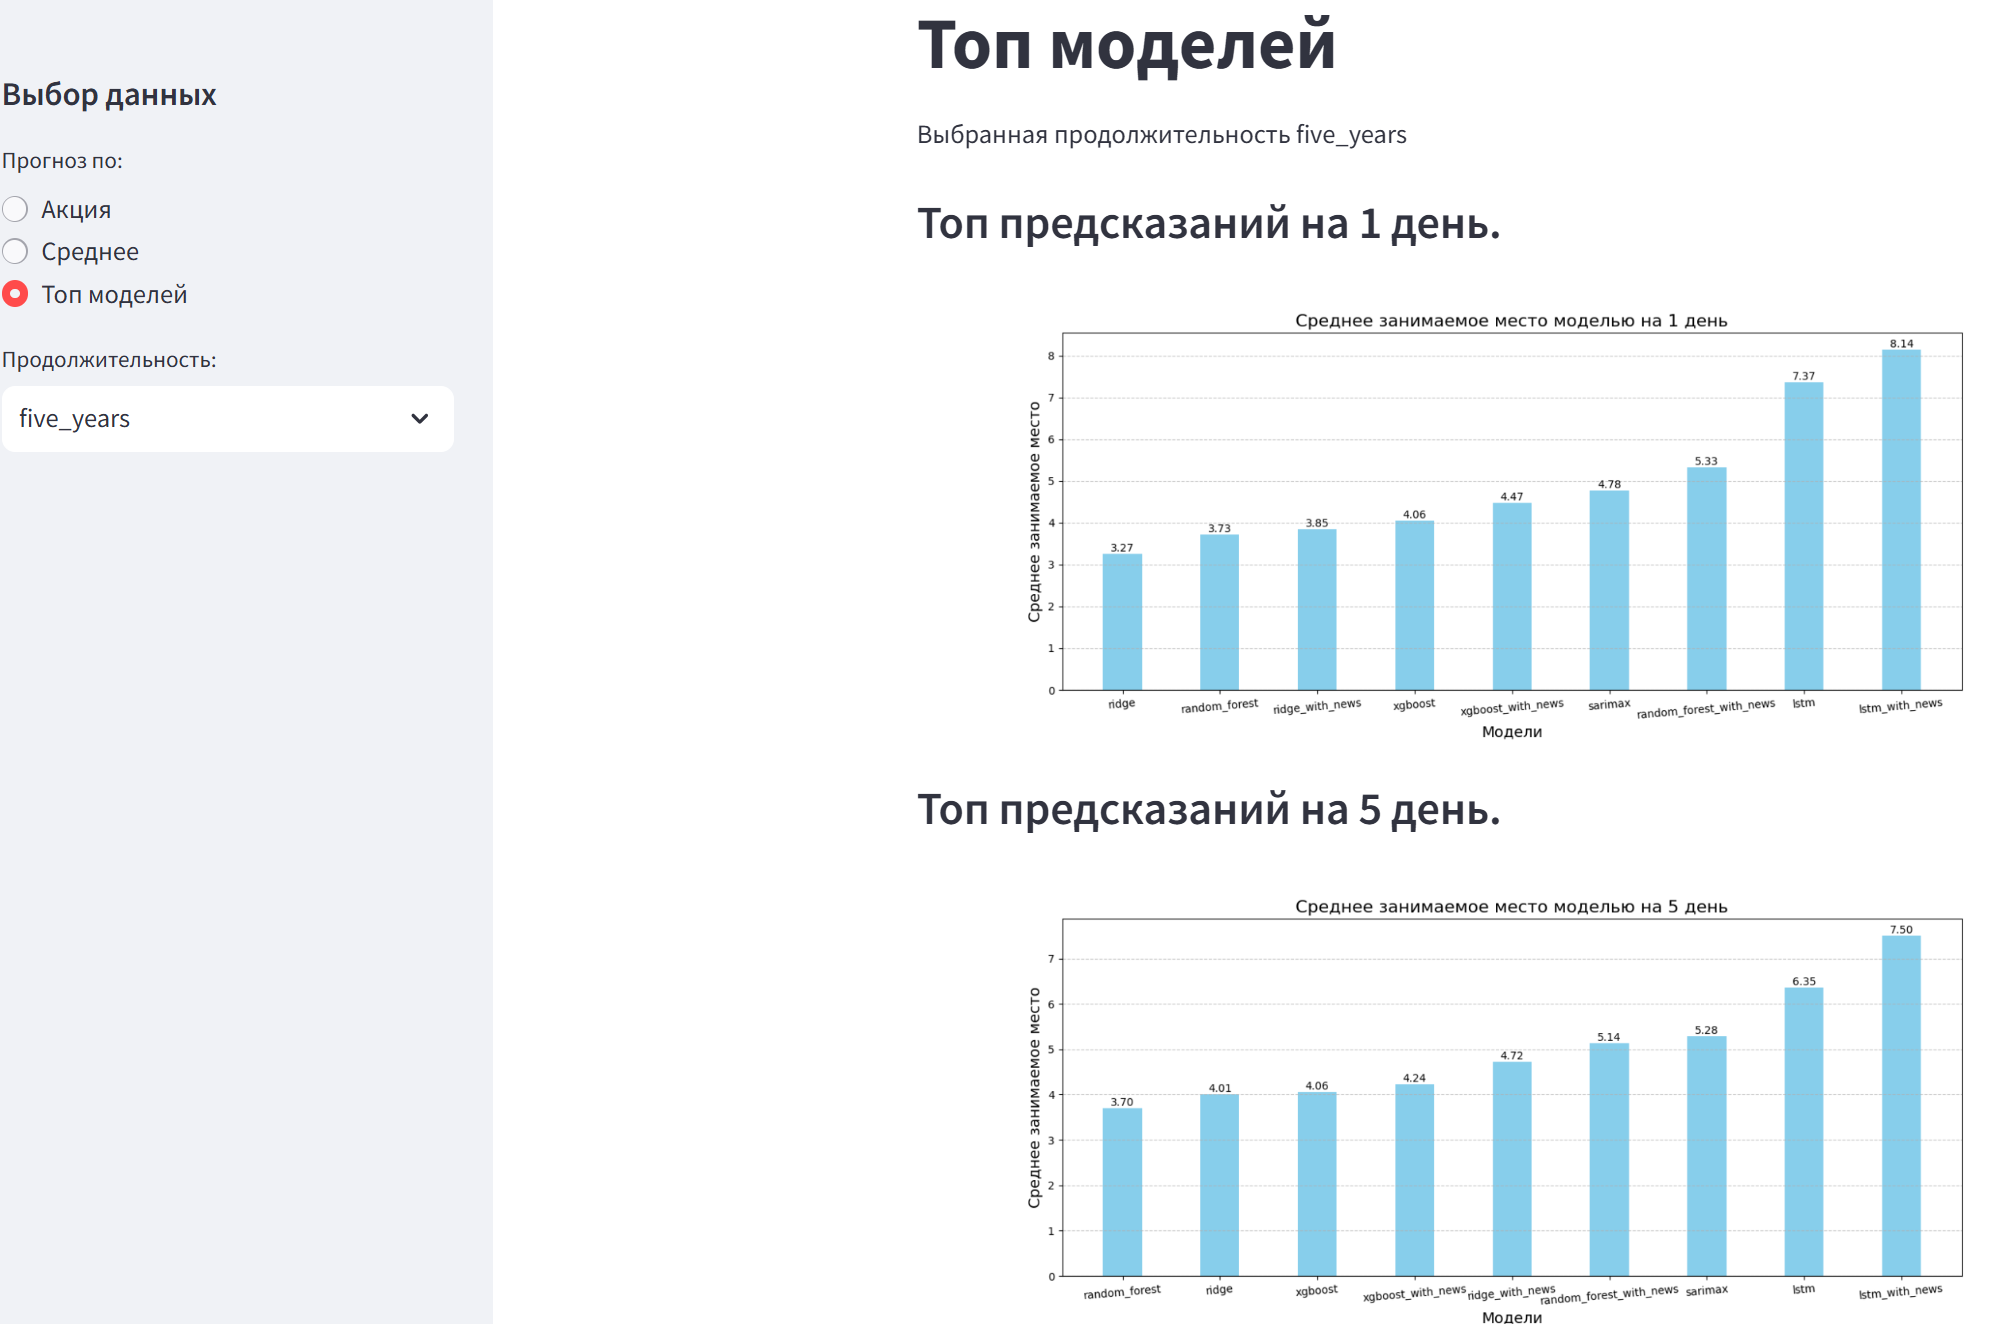
\includegraphics[width=1\linewidth]{top}}
\caption{Страница топа моделей на коротком горизонте.}
\label{fig:top}
\end{figure}
\begin{figure}[!h]
\center{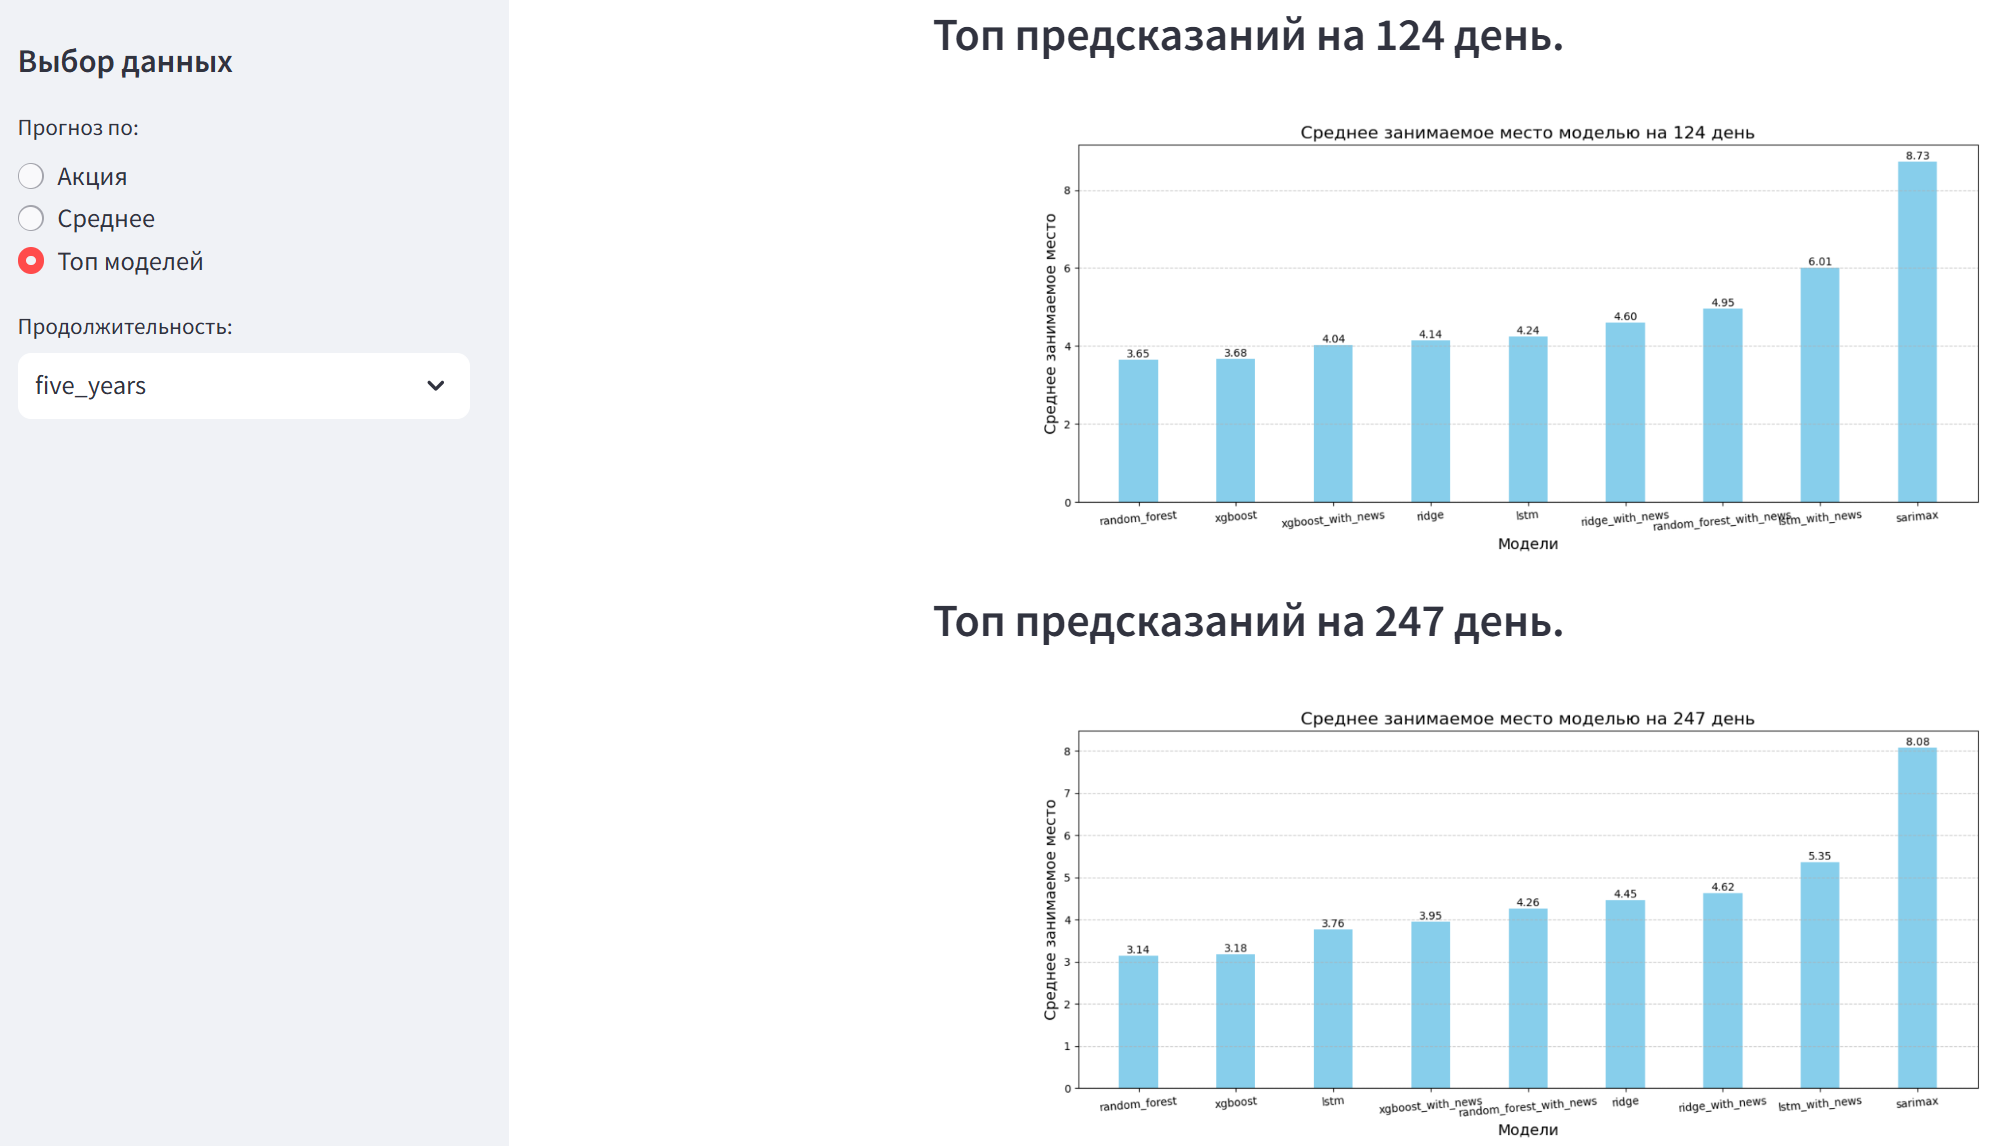
\includegraphics[width=1\linewidth]{top_other}}
\caption{Страница лучших моделей на длинном горизонте.}
\label{fig:top_other}
\end{figure}

\section{Как можно улучшить результат}

Для получения более точных прогнозов я вижу несколько вариантов.

Первое. Лучше выбирать бумаги, в которых вы лучше разбираетесь, то есть иметь экспертизу в той области, в которой работает компания. Это поможет вам самим понять, правдоподобен ли прогноз, учитывая текущее состояник компании, её окружение и менеджмент. Верите ли вы в такое и насколько соответствует вашему риск-профилю.

Второе. По возможности увеличивать количество данных по её цене, чтобы тренировочных данных было много. И постараться более здраво заполнять имеющиеся пропуски.

Третье. Использовать больше данных. Добавлять в модели параметры EBITDA, P/E и другие. Использовать известные дневные минимальные и максимальные цены, объём торгов и их стоимость.

Четвёртое. Лучше и точнее определять новостной фон. Учитывать, что по общим новостям тяжелее выявлять информацию о мелких или непопулярных компаниях. Возможно, лучше дополнять новостями для конкретных эмитентов.

Пятое. Попробовать подобрать параметры моделей лучше и построить более хорошую LSTM-модель.

\section{Заключение}

В заключение моего исследования хотелось бы отметить, что в рамках данной выпускной квалификационной работы мною были собраны, обработаны, проанализированы и подготовлены данные по 215 акциям и более чем 2 млн. новостей. Были обучены такие модели, как SARIMAX, Ridge, Random Forest, XGBoost и LSTM. Результаты были проанализированы и представлены в удобном формате в виде сервиса, как по отдельным бумагам, так и средние показатели для получения общей картины.

Результы работы следующие. Лучшей моделью оказался случайный лес, он проигрывает Ridge только на начальном этапе, но уже через пару дней показывает более точные прогнозы. Кроме того, он является более устойчивым на большем горизонте. Также градиентный бустинг очень хорош, из полученных результатов видно, что данная модель немного хуже случайного леса, но все равно достаточно точна и тоже более стабильна в будущем. По поводу ARIMA-подобных моделей, не думаю, что они достаточно конкурентоспособны по сравнению с остальными. А LSTM в моей работе выглядит наиболее стабильной, но не столь точной, вполне возможно, что при построении хорошей нейронной сети результаты будут более точными.

Хотя в среднем модели с использованием новостей показали результат немного хуже, чем без них, я считаю, что новостные данные положительно влияют на результаты моделей, потому что они часто показывали хороший результат. Только для этого я бы советовал собирать как можно больше данных для вашей акции. Чем больше новостей, влияющих на ваши бумаги, вы сможете найти, тем больше информации модель сможет из этих данных получить. Если новостных данных по эмитенту не так много, то лучше рассматривать модели без использования новостей.

И напоследок, хотел бы сказать, что не стоит слепо верить прогнозам моделей, тем более на большом горизонте. Лучше стабильно инвестировать, а не пытаться предугадать, что произойдет на рынке завтра, ведь рано или поздно все пойдет не по плану. Рынок резко рухнет или поднимется, что предугадать невозможно. Вы определенно не успеете среагировать, что может привести к проблемам. Но, не пытаясь переиграть рынок и имея стратегию, вы будете готовы к любым взлётам и падениям.

\newpage
\printbibliography
\addcontentsline{toc}{section}{Список литературы}
\end{document}